\NoBgThispage
\chapter{MapAlign: Training and Model Approaches}

This chapter provides a detailed and comprehensive analysis of the developed architecture throughout its various phases, focusing particularly on the two approaches that reached the most promising results.

\section{First Approach}

The first approach aimed to create a model to perform the task explained earlier without using raw images. Instead, it used features extracted by neural network detectors running directly on the car. These detectors captured information like curbs, markings, and boundaries from image sequences and stored it in the packed data described before. This made the input much smaller since the raw image data was not included.

The \textit{BEVPreprocessor} prepares the input data with a simple structure consisting of a single convolutional layer with just $0.0013$ million parameters, keeping it efficient. 
The \textit{Backbone}, based on the BiSeNetV1 architecture \cite{DBLP:journals/corr/abs-1808-00897}, is the most complex component, with $12.63$ million parameters. The backbone uses two paths: 
\begin{enumerate}
    \item Spatial Path: Designed with a small stride to preserve spatial details, this path captures high-resolution features through several convolutional layers, emphasizing fine-grained spatial information.
    \item Context Path: This path quickly down-samples the input to expand the receptive field, helping the model capture broader context. It utilizes Attention Refinement Modules (ARMs) and additional convolutional layers. ARMs allow the model to focus on important regions within the image, significantly contributing to the model's parameter count.
\end{enumerate}
A Feature Fusion Module is used to efficiently combine the features from the Spatial and Context Paths.

The \textit{Decoder} then up-samples these features to restore them to the original input resolution, with a parameter count of $0.0924$ million. The role of the decoder is to convert high-level, low-resolution features back into the detailed, high-resolution format needed for accurate output. This component ensures that the model’s outputs match the input image's scale, making the model suitable for precise localization tasks.

The head, called \textit{PoseSegHead}, generates the segmentation output, while a fully connected (Fc) layer finalizes the pose estimation. This design enables efficient and accurate pose analysis. The model’s total parameter count is optimized to balance processing efficiency and accuracy.

Figure \ref{fig:enter-label12} illustrates the complete model structure.
\begin{figure}[H]
    \centering
    \includegraphics[width=0.75\linewidth]{LateX//figs/modello_POSENET.pdf}
    \caption{Structure of the PoseNet Model INSERIRE SCHEMA}
    \label{fig:enter-label12}
\end{figure}

The primary goal was to accurately predict the four values that allow the alignmente between the car pose and the HD map: translations along the \( x, y, z \) axes and the heading angle. Alongside model design, appropriate loss functions were also defined. As described in Chapter 1, the three loss functions used were L1, L1-smooth, and MSE.
It is advantageous to employ a single loss function that accounts for all parameters collectively, as this ensures the network learns to optimize the relationships and trade-offs between them in a holistic manner. However, incorporating individual loss components for each parameter can further enhance the model's performance by encouraging it to focus on specific prediction tasks. This approach can improve interpretability, as it allows the network to account for parameter-specific nuances, and promote generalization by preventing the dominance of any single parameter in the optimization process. For this reason two additional specialized losses for the translation and heading angle were added. 
The heading angle was especially critical and challenging to learn accurately, so this structure was consistent across different model versions.

The initial iterations used the following high-level parameters:
\begin{itemize}
    \item Data augmentation: Included body rotations between $-30^\circ$ and $30^\circ$, and horizontal and vertical shifts up to $10\%$.
    \item Optimizer: Training used the SGD optimizer with a base learning rate of \textit{0.1} and a batch size of \textit{64}.
    \item Learning Rate Scheduler: The scheduler was WarmupPolyLR \cite{kalra2024warmuplearningrateunderlying} with a warm-up period of $5000$ iterations, capped at a maximum of $100000$ iterations.
    \item Automatic Mixed Precision (AMP) was enabled to improve training speed and resource use.
\end{itemize}

The learning rate demonstrated the following behavior during training:
\begin{figure}[H]
    \centering
    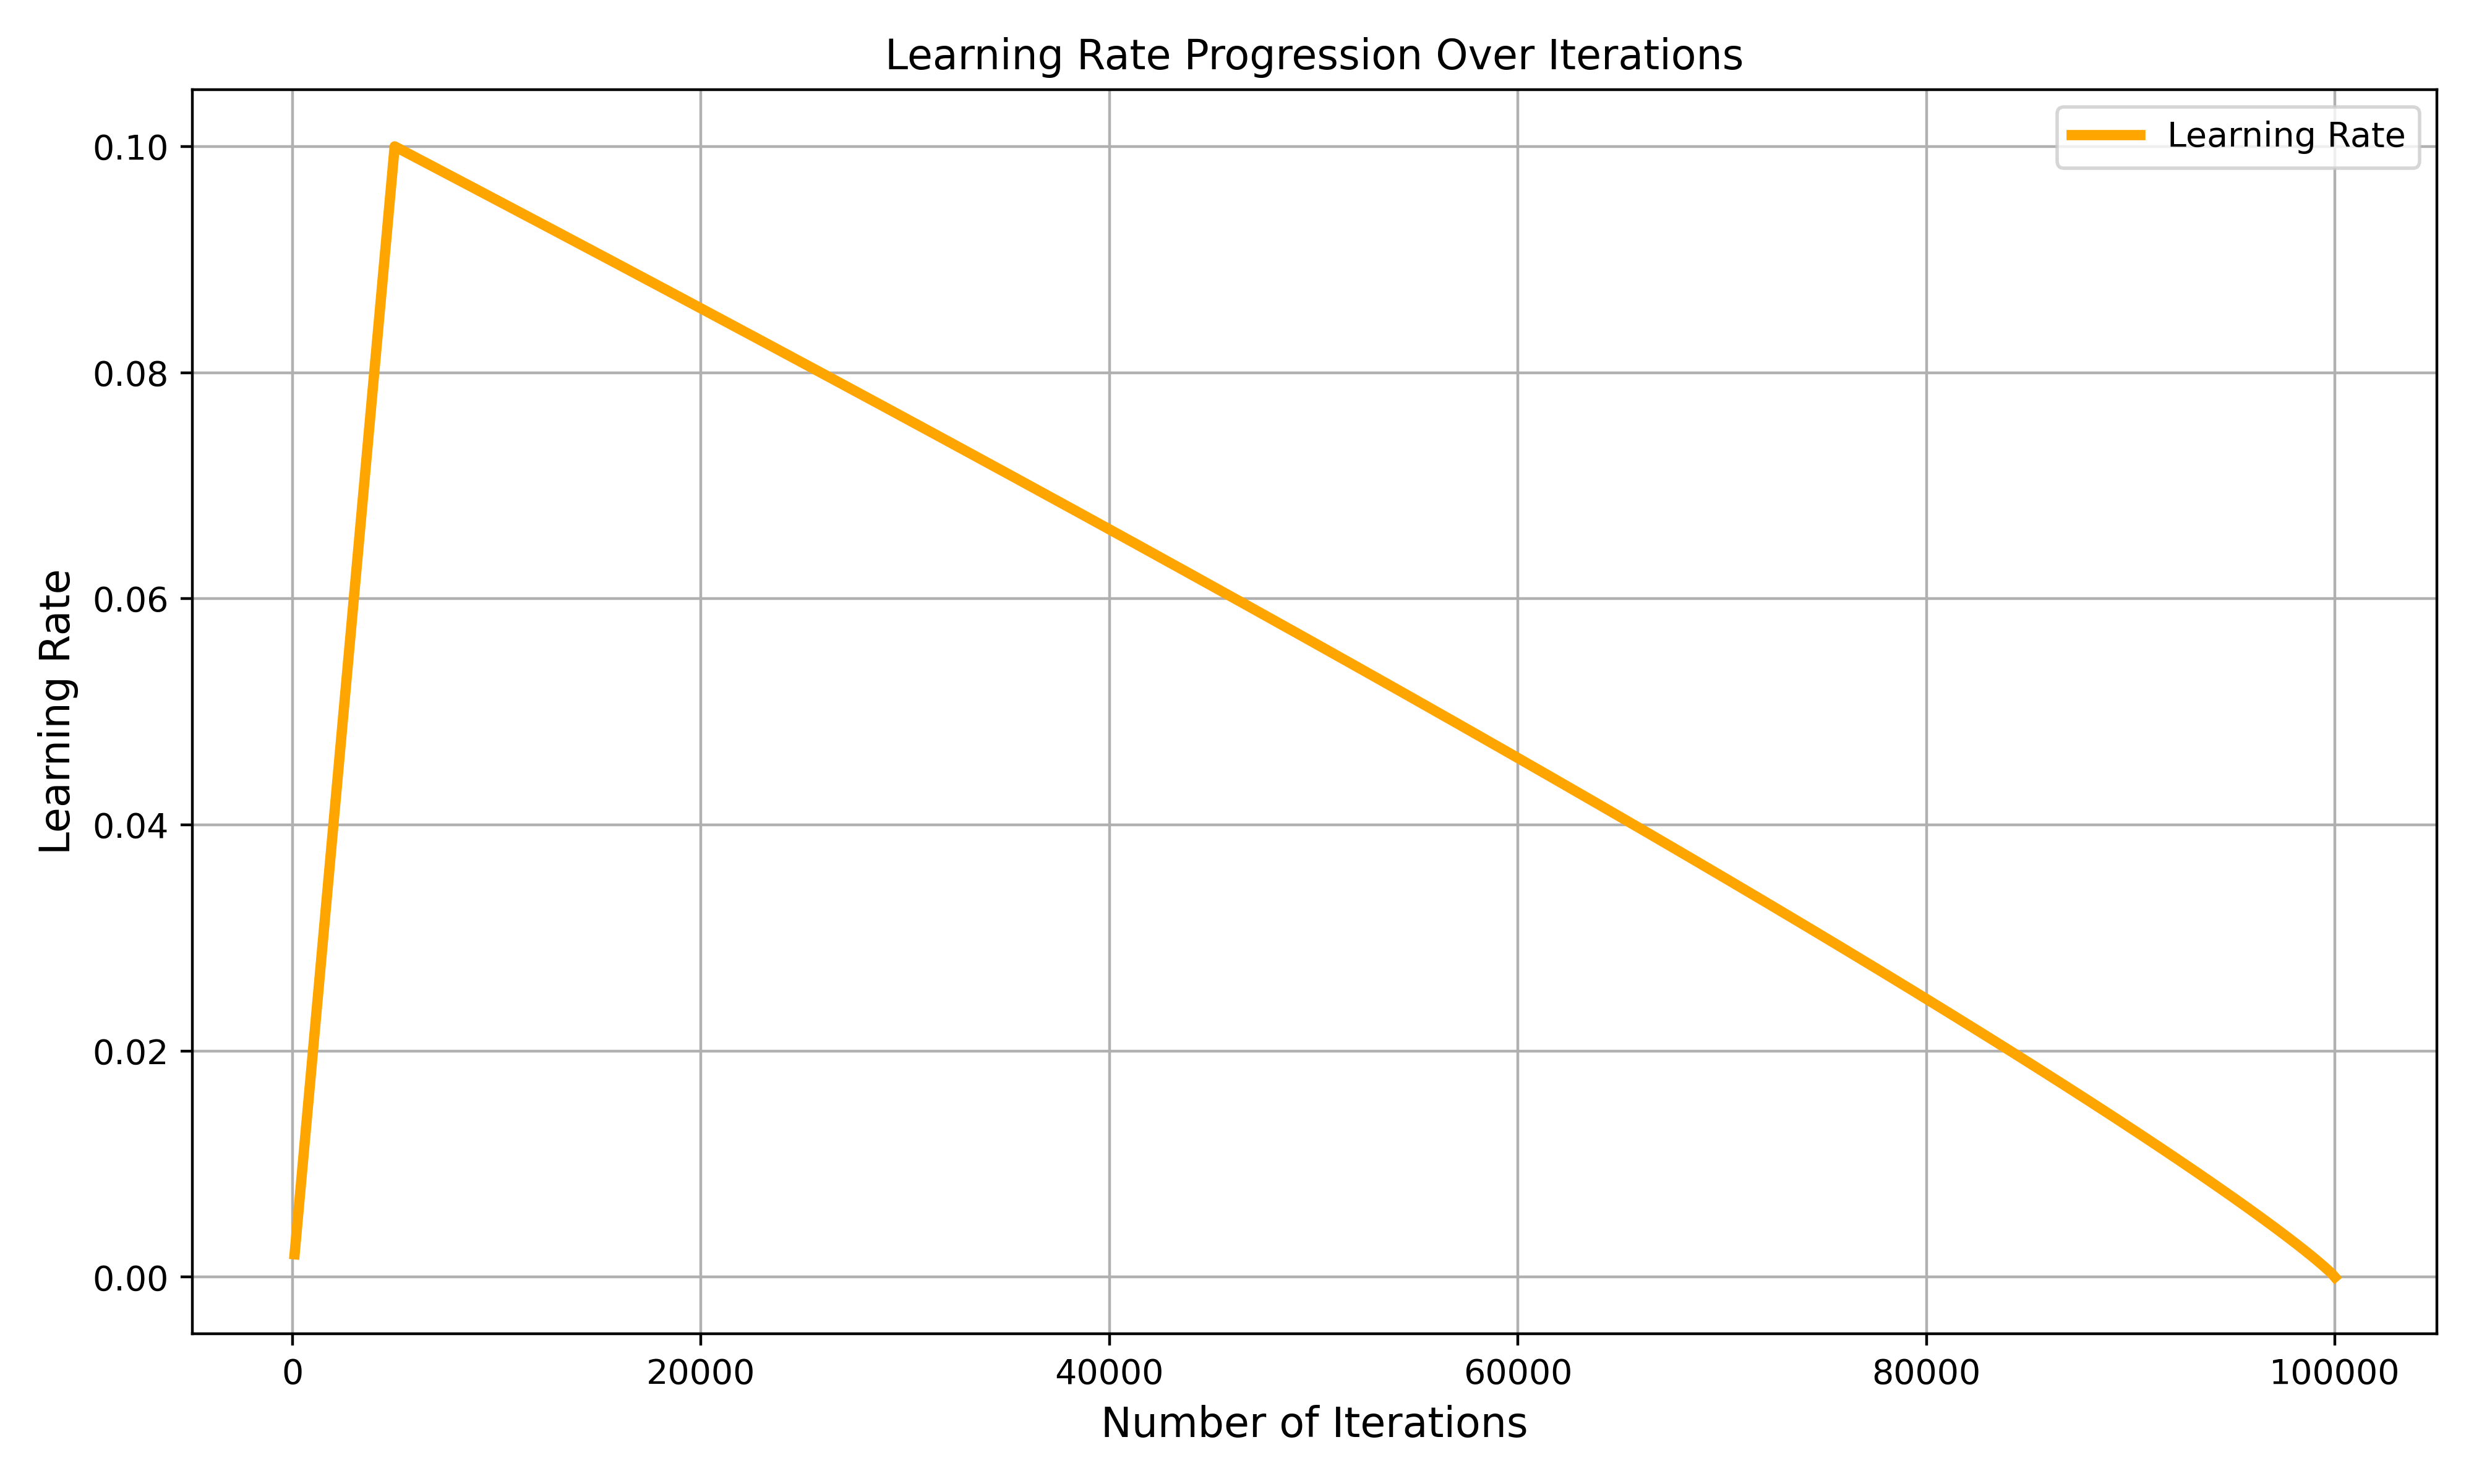
\includegraphics[width=0.75\linewidth]{LateX//figs/learning_rate_progression.png}
    \caption{Learning Rate Progression During Training}
    \label{fig:learning-rate-progression}
\end{figure}

Checkpoints were saved every $100$ iterations, and evaluations were performed every $5000$ iterations using the \textit{PoseEvaluator}. The evaluator calculated the L1 loss on a validation set to objectively assess the model’s performance. The loss was computed as the absolute difference between the ground truth and predicted values for position and heading, as shown below:
\begin{align}
    \text{eval}_x &= |x_{\text{gt}} - x_{\text{pred}}|, \\
    \text{eval}_y &= |y_{\text{gt}} - y_{\text{pred}}|, \\
    \text{eval}_z &= |z_{\text{gt}} - z_{\text{pred}}|, \\
    \text{eval}_{\theta} &= |\theta_{\text{gt}} - \theta_{\text{pred}}|.
\end{align}

Training was accelerated with CUDA, using CuDNN benchmarking for improved speed. Initial training sessions utilized only a portion of the dataset to refine the model’s structure and functionality before scaling to the full dataset.

\subsubsection*{MSE}
The first training session of the architecture described used MSE as the loss function, along with the parameters described above. This approach resulted in a steadily decreasing loss, as shown in the figure below:
\begin{figure}[H]
    \centering
    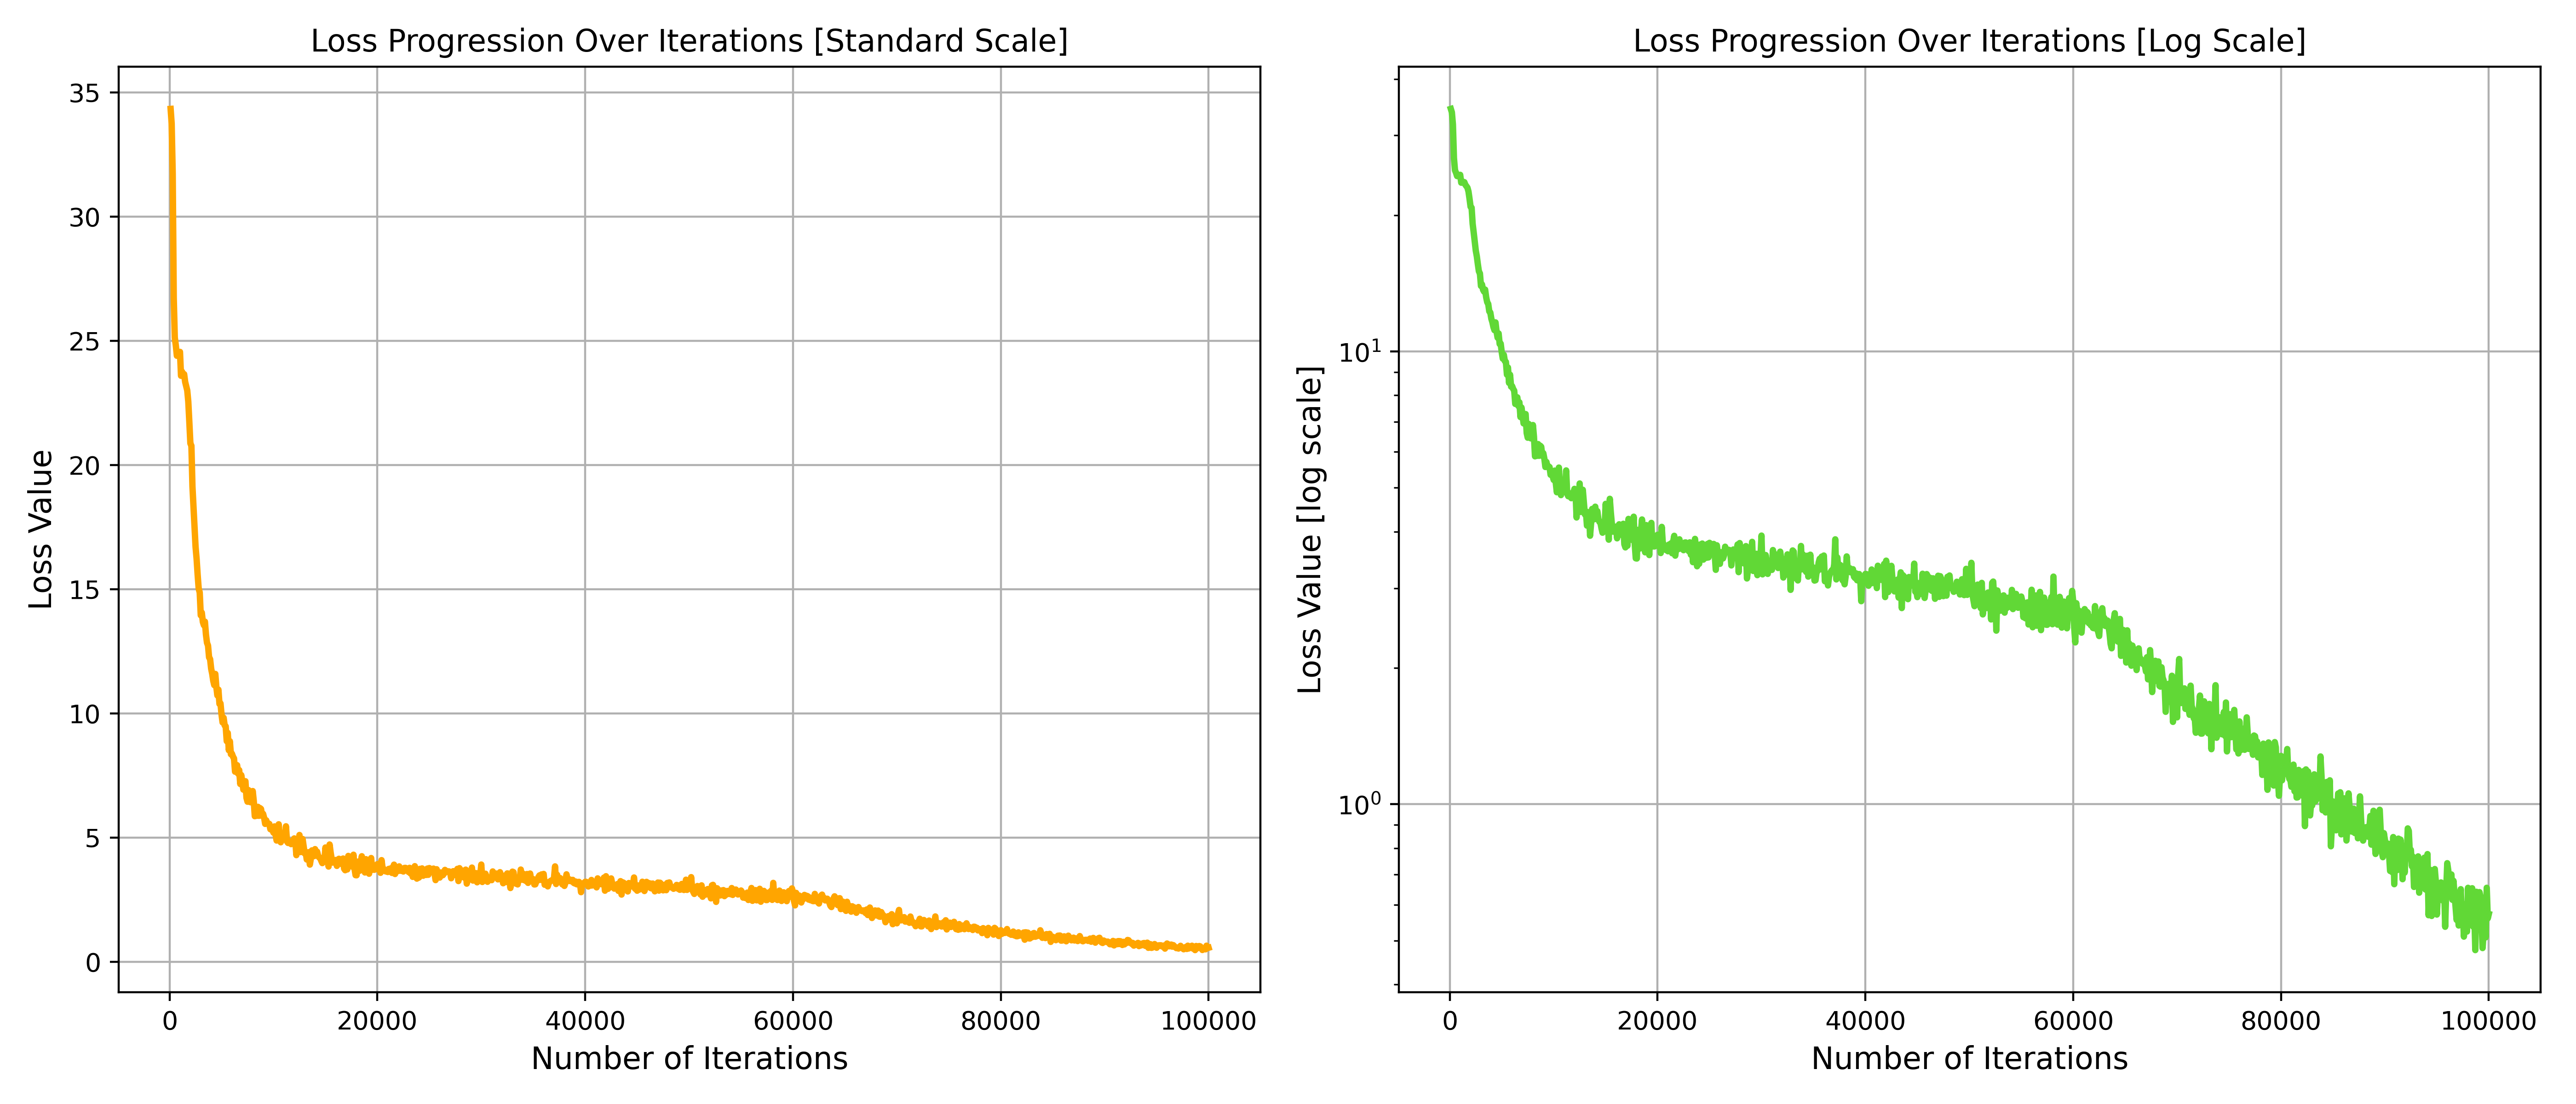
\includegraphics[width=1\linewidth]{LateX//figs/loss_total_mse_progression_comparison.png}
    \caption{Total Loss Progression Using MSE as the Loss Function}
    \label{fig:mse-loss-progression}
\end{figure}

Focusing on specific losses for the pose and heading angle, the following behavior was observed:
\begin{figure}[H]
    \centering
    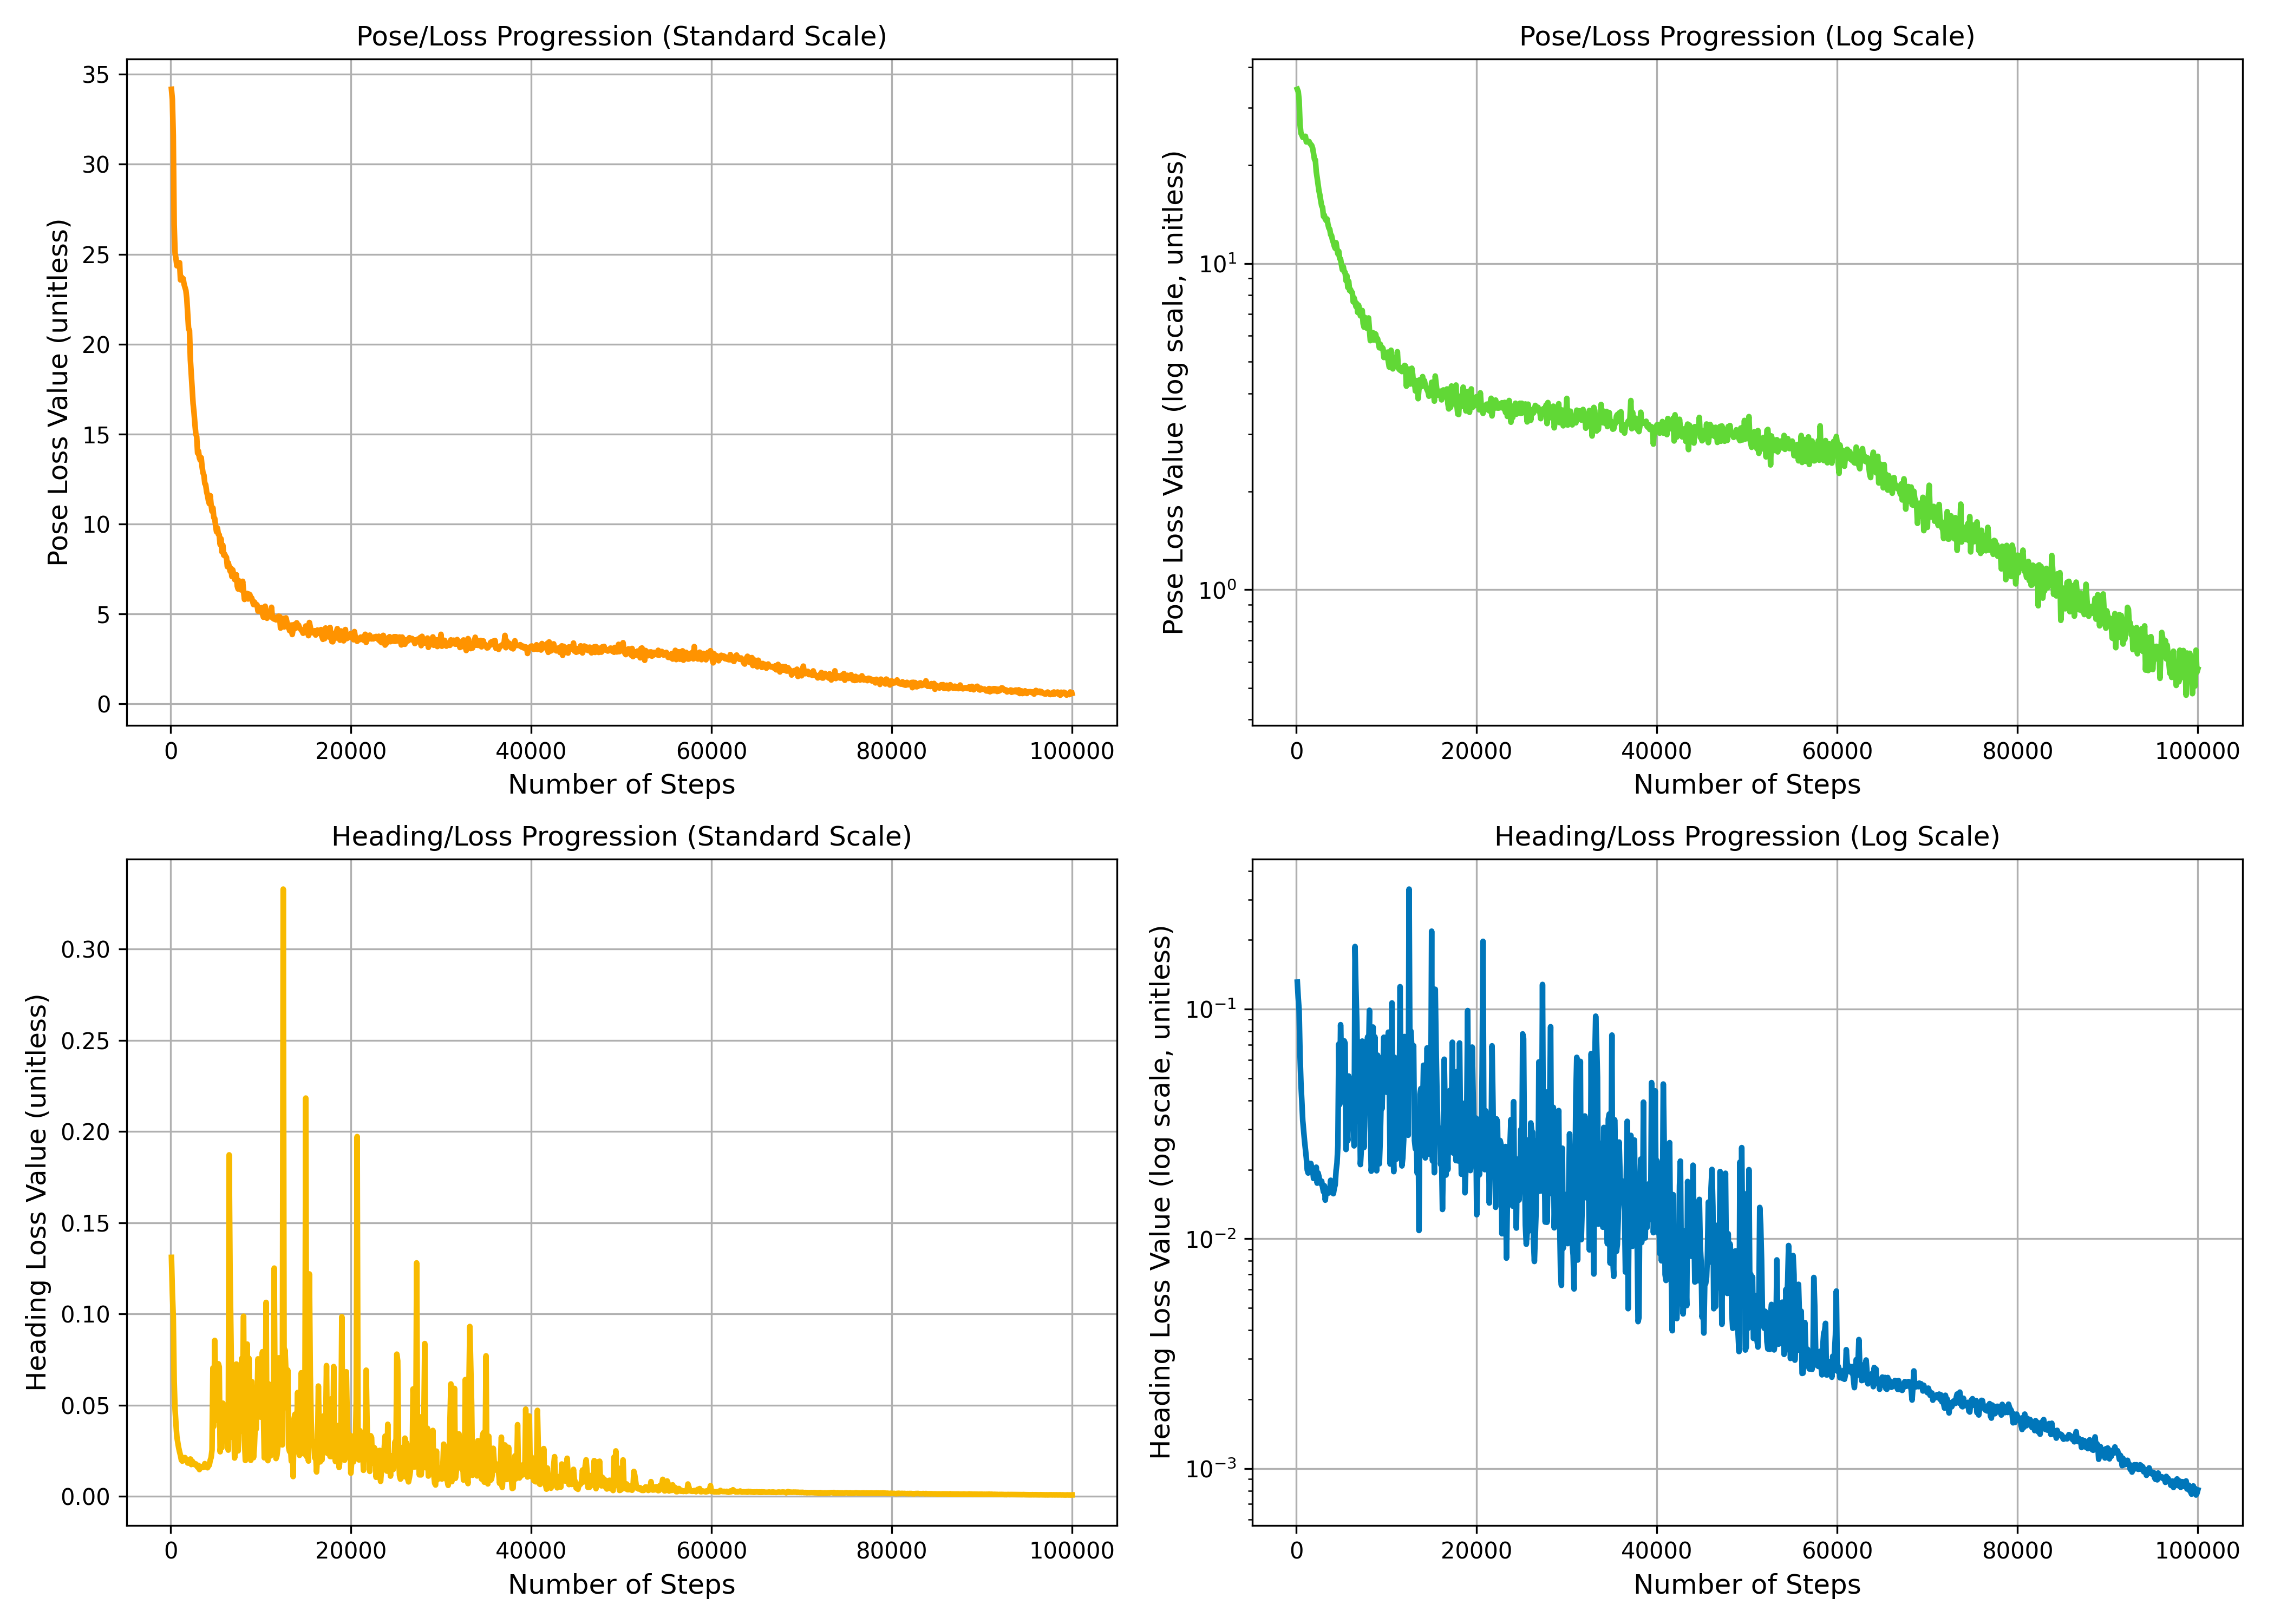
\includegraphics[width=1\linewidth]{LateX//figs/mse_pose_heading_loss_comparison.png}
    \caption{Pose and Heading Loss Comparison During Training}
    \label{fig:pose-heading-loss}
\end{figure}

The model's behavior during evaluation aligned with expectations, and the training evaluations yielded the following results:
\begin{table}[H]
    \centering
    \begin{tabular}{>{\centering\arraybackslash}p{2.25cm} >{\centering\arraybackslash}p{2.25cm} >{\centering\arraybackslash}p{3.25cm} >{\centering\arraybackslash}p{2.25cm} >{\centering\arraybackslash}p{2.25cm}}
        \toprule
        \textbf{Iteration} & \textbf{$\Delta$ Pose} & \textbf{$\Delta \theta$} & \textbf{$\Delta x + \Delta y$} & \textbf{$\Delta h$} \\
        & \text{[m]} & \text{[rad] $\rightarrow$ [deg]} & \text{[m]} & \text{[m]} \\
        \midrule
        \num{20000} & 2.02 & 0.05 $\rightarrow$ 2.86 & 1.94 & 0.08 \\
        \num{40000} & 1.43 & 0.22 $\rightarrow$ 12.6 & 1.37 & 0.06 \\
        \num{60000} & 1.42 & 0.04 $\rightarrow$ 2.29 & 1.39 & 0.02 \\
        \num{80000} & 1.99 & 0.02 $\rightarrow$ 1.15 & 1.99 & 0.00 \\
        \num{100000} & 1.54 & 0.02 $\rightarrow$ 1.15 & 1.54 & 0.00 \\
        \bottomrule
    \end{tabular}
    \caption{Variations in pose, angle, xy, and height across different iterations.}
    \label{tab:pose_variations}
\end{table}

Despite the loss functions decreasing and reaching very low values, indicating potential generalization and effective learning, the evaluation process reveals that the results are still not optimal or acceptable. The positional error exceeds one meter, which is insufficient for HD map alignment applications, as discussed in Chapter 1. This could be acceptable if iterative optimization is still included in the desired pipeline of the dataset generator. This approach could simply eliminate the part where the sequences had to be manually aligned. However, it was not sufficient, so other attempts were made and will be further demonstrated. 

\subsection*{L1 Loss}
In this other example, the total loss was supplemented by two specific auxiliary losses using the L1 loss, defined similarly to the previous set-up. The results with the L1 loss are consistent with previous observations. 
The figure below illustrates the behavior of the neural network. Vertically, the first three images represent the inputs: obstacles extracted directly on the car, associated HD maps, and the fusion of the two. The fourth image represents the target, which is the perfect alignment that the network aims to achieve. The last image represents the prediction by the network. As can be seen, this time, the prediction is post-processed to perform a roto-translation of the car and its world reconstruction.

The results show measurements taken at two different points during training: one at the start and one close to the end. At the start, the network doesn't provide right values as it has not yet learned to generalize well. By the end of training, the second figure shows that the network's performance improves significantly, and the misalignments decrease a lot, though they do not reach zero.
\begin{figure}[H]
    \centering
    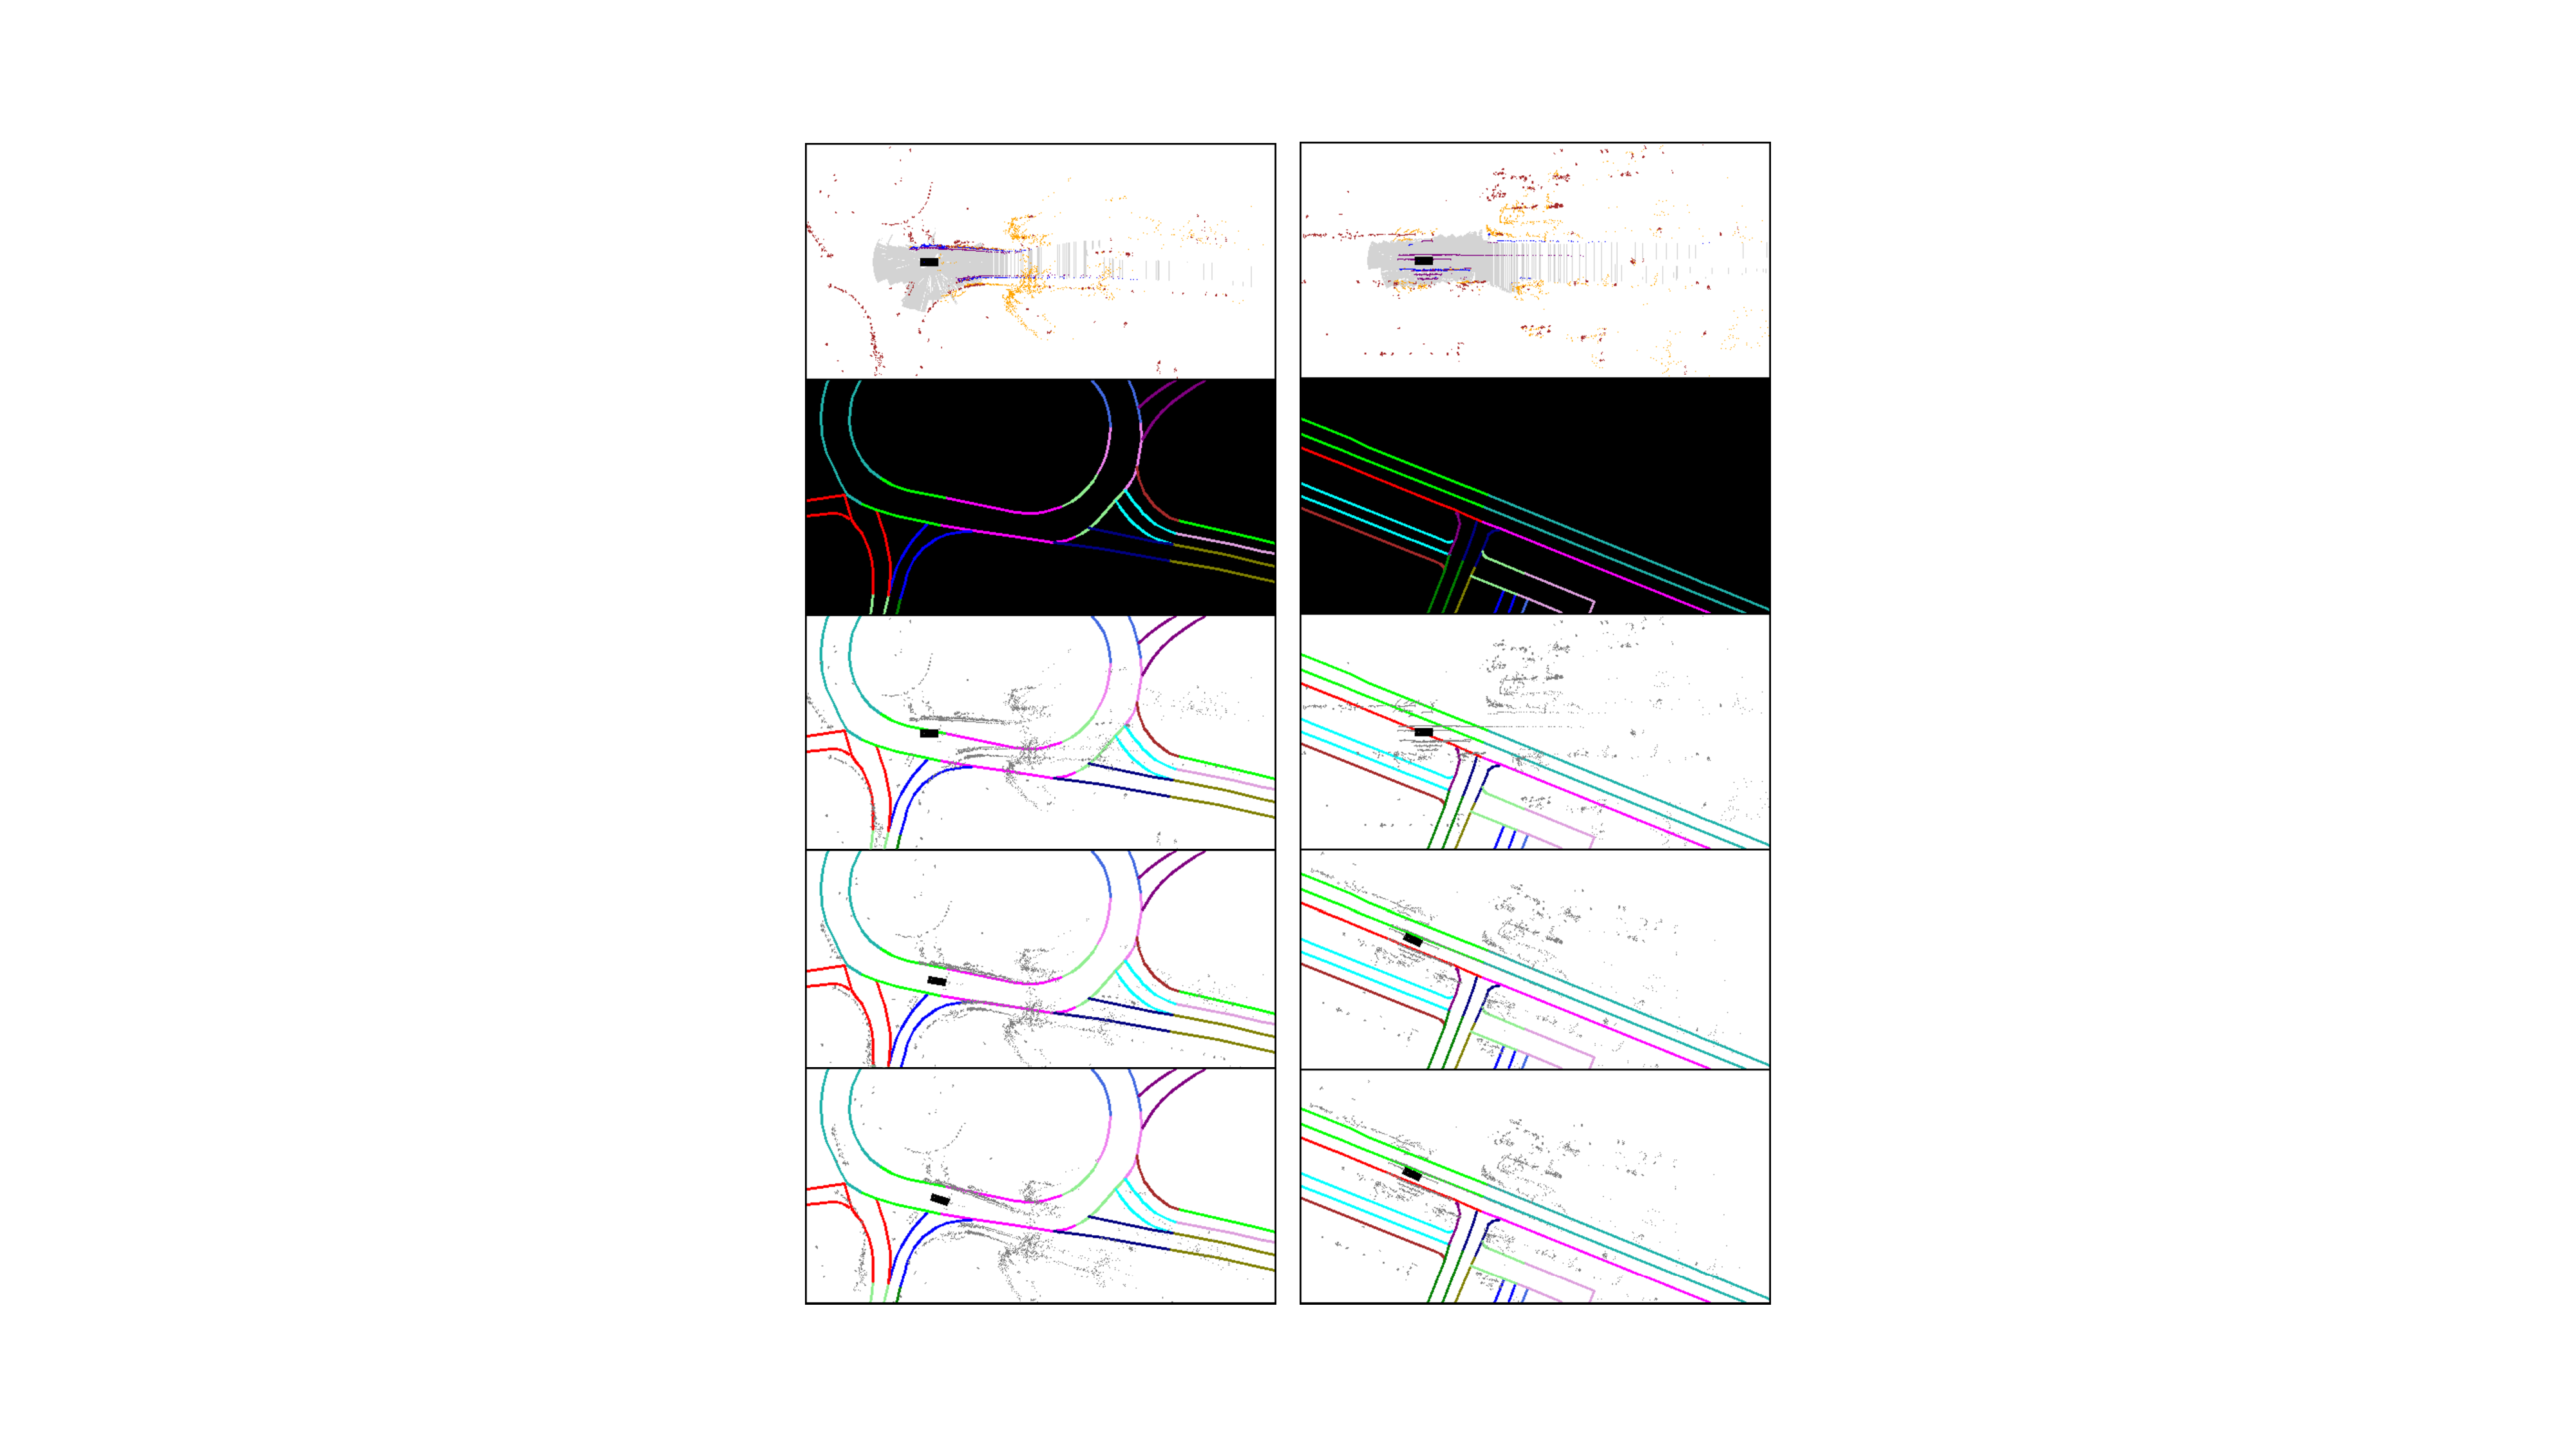
\includegraphics[width=1\linewidth]{LateX//figs/IMMAGINI_L1_rete.pdf}
    \caption{Enter Caption}
    \label{fig:enter-label}
\end{figure}

Since the specific loss graphs didn’t show any significant differences, only the results table is presented for this experiment.
\begin{table}[H]
    \centering
    \begin{tabular}{>{\centering\arraybackslash}p{2.25cm} >{\centering\arraybackslash}p{2.25cm} >{\centering\arraybackslash}p{3.25cm} >{\centering\arraybackslash}p{2.25cm} >{\centering\arraybackslash}p{2.25cm}}
        \toprule
        \textbf{Iteration} & \textbf{$\Delta$ Pose} & \textbf{$\Delta \theta$} & \textbf{$\Delta x + \Delta y$} & \textbf{$\Delta h$} \\
        & \text{[m]} & \text{[rad] $\rightarrow$ [deg]} & \text{[m]} & \text{[m]} \\
        \midrule
        \num{20000} & 2.00 & 0.11 $\rightarrow$ 6.31 & 1.98 & 0.02 \\
        \num{40000} & 1.89 & 0.13 $\rightarrow$ 7.45 & 1.84 & 0.05 \\
        \num{60000} & 1.45 & 0.04 $\rightarrow$ 2.29 & 1.43 & 0.02 \\
        \num{80000} & 1.42 & 0.04 $\rightarrow$ 2.29 & 1.40 & 0.02 \\
        \num{100000} & 1.40 & 0.03 $\rightarrow$ 1.72 & 1.40 & 0.00 \\
        \bottomrule
    \end{tabular}
    \caption{Variations in pose, angle, xy, and height across different iterations.}
    \label{tab:pose_variations}
\end{table}
On the small test set, it’s evident that simply changing the loss function to L1 is insufficient to achieve the required precision to eliminate the iterative optimizer. 

\subsection*{Smooth L1 Loss}
In this experiment, the Smooth L1 loss, which is similar to L1 but less sensitive to outliers, was employed. The training results, as expected, remained consistent. However, this time, some interesting differences emerged. The results demonstrated slight improvements compared to previous attempts. Both loss graphs and the evaluation table are provided below to illustrate this behavior.

The total loss graph exhibits the anticipated behavior, gradually decreasing as the number of iterations increases. 
\begin{figure}[H]
    \centering
    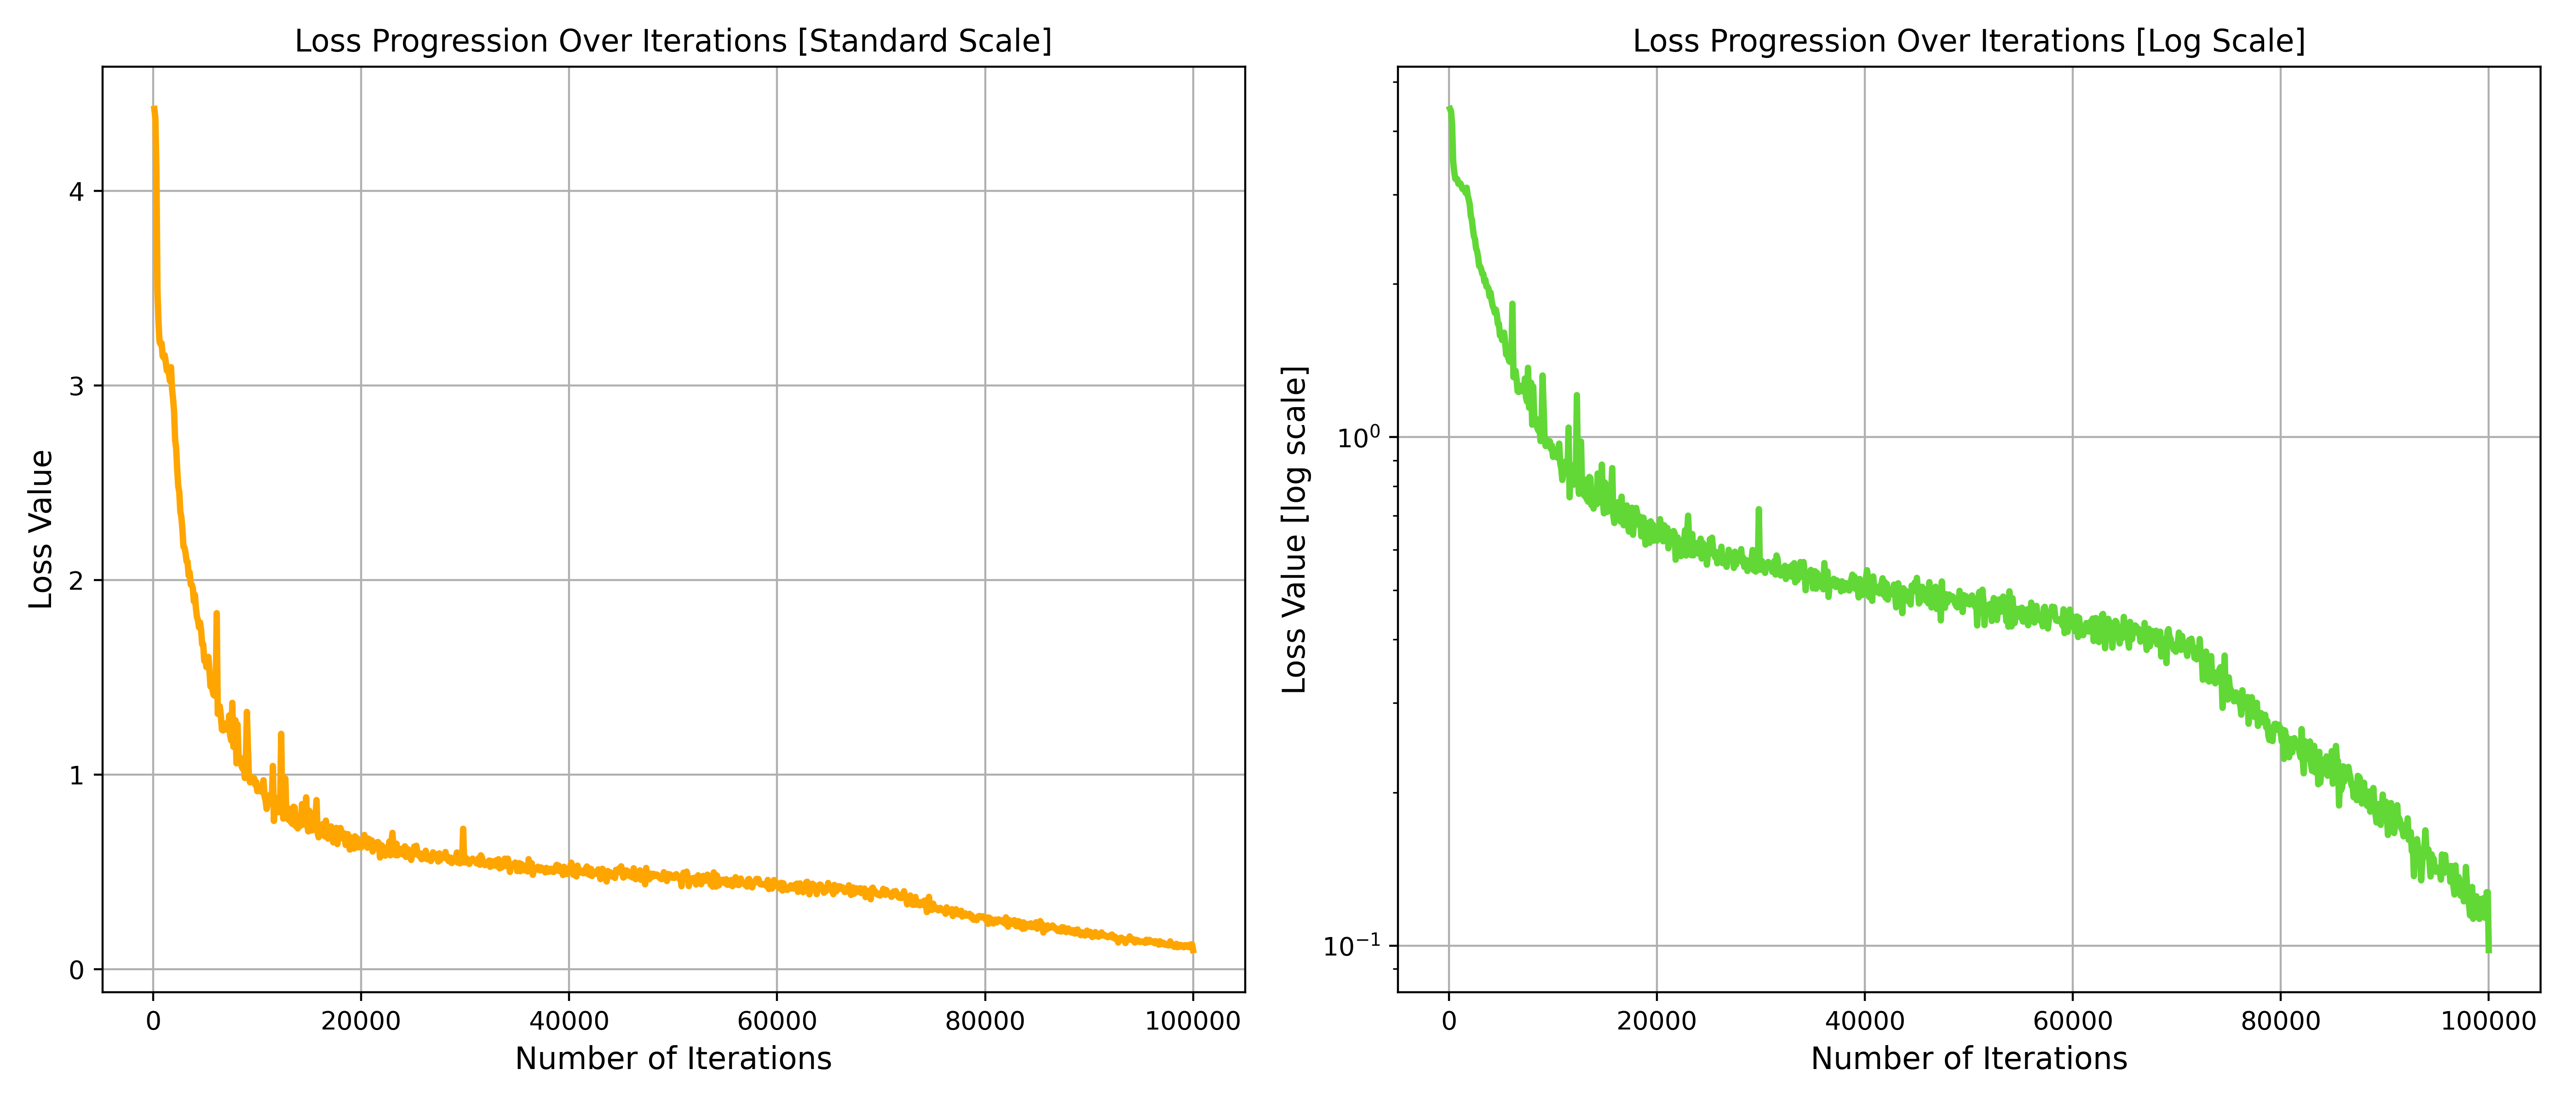
\includegraphics[width=1\linewidth]{LateX//figs/loss_total_l1s_progression_comparison.png}
    \caption{Total Loss Progression Using Smooth L1 Loss}
    \label{fig:smooth-l1-total-loss}
\end{figure}

As shown in the figure, the total loss contributions reveal that the translation component constitutes the majority, while the heading loss contributes only a minor portion to the overall result. This observation prompted further investigation into this behavior in following experiments.
\begin{figure}[H]
    \centering
    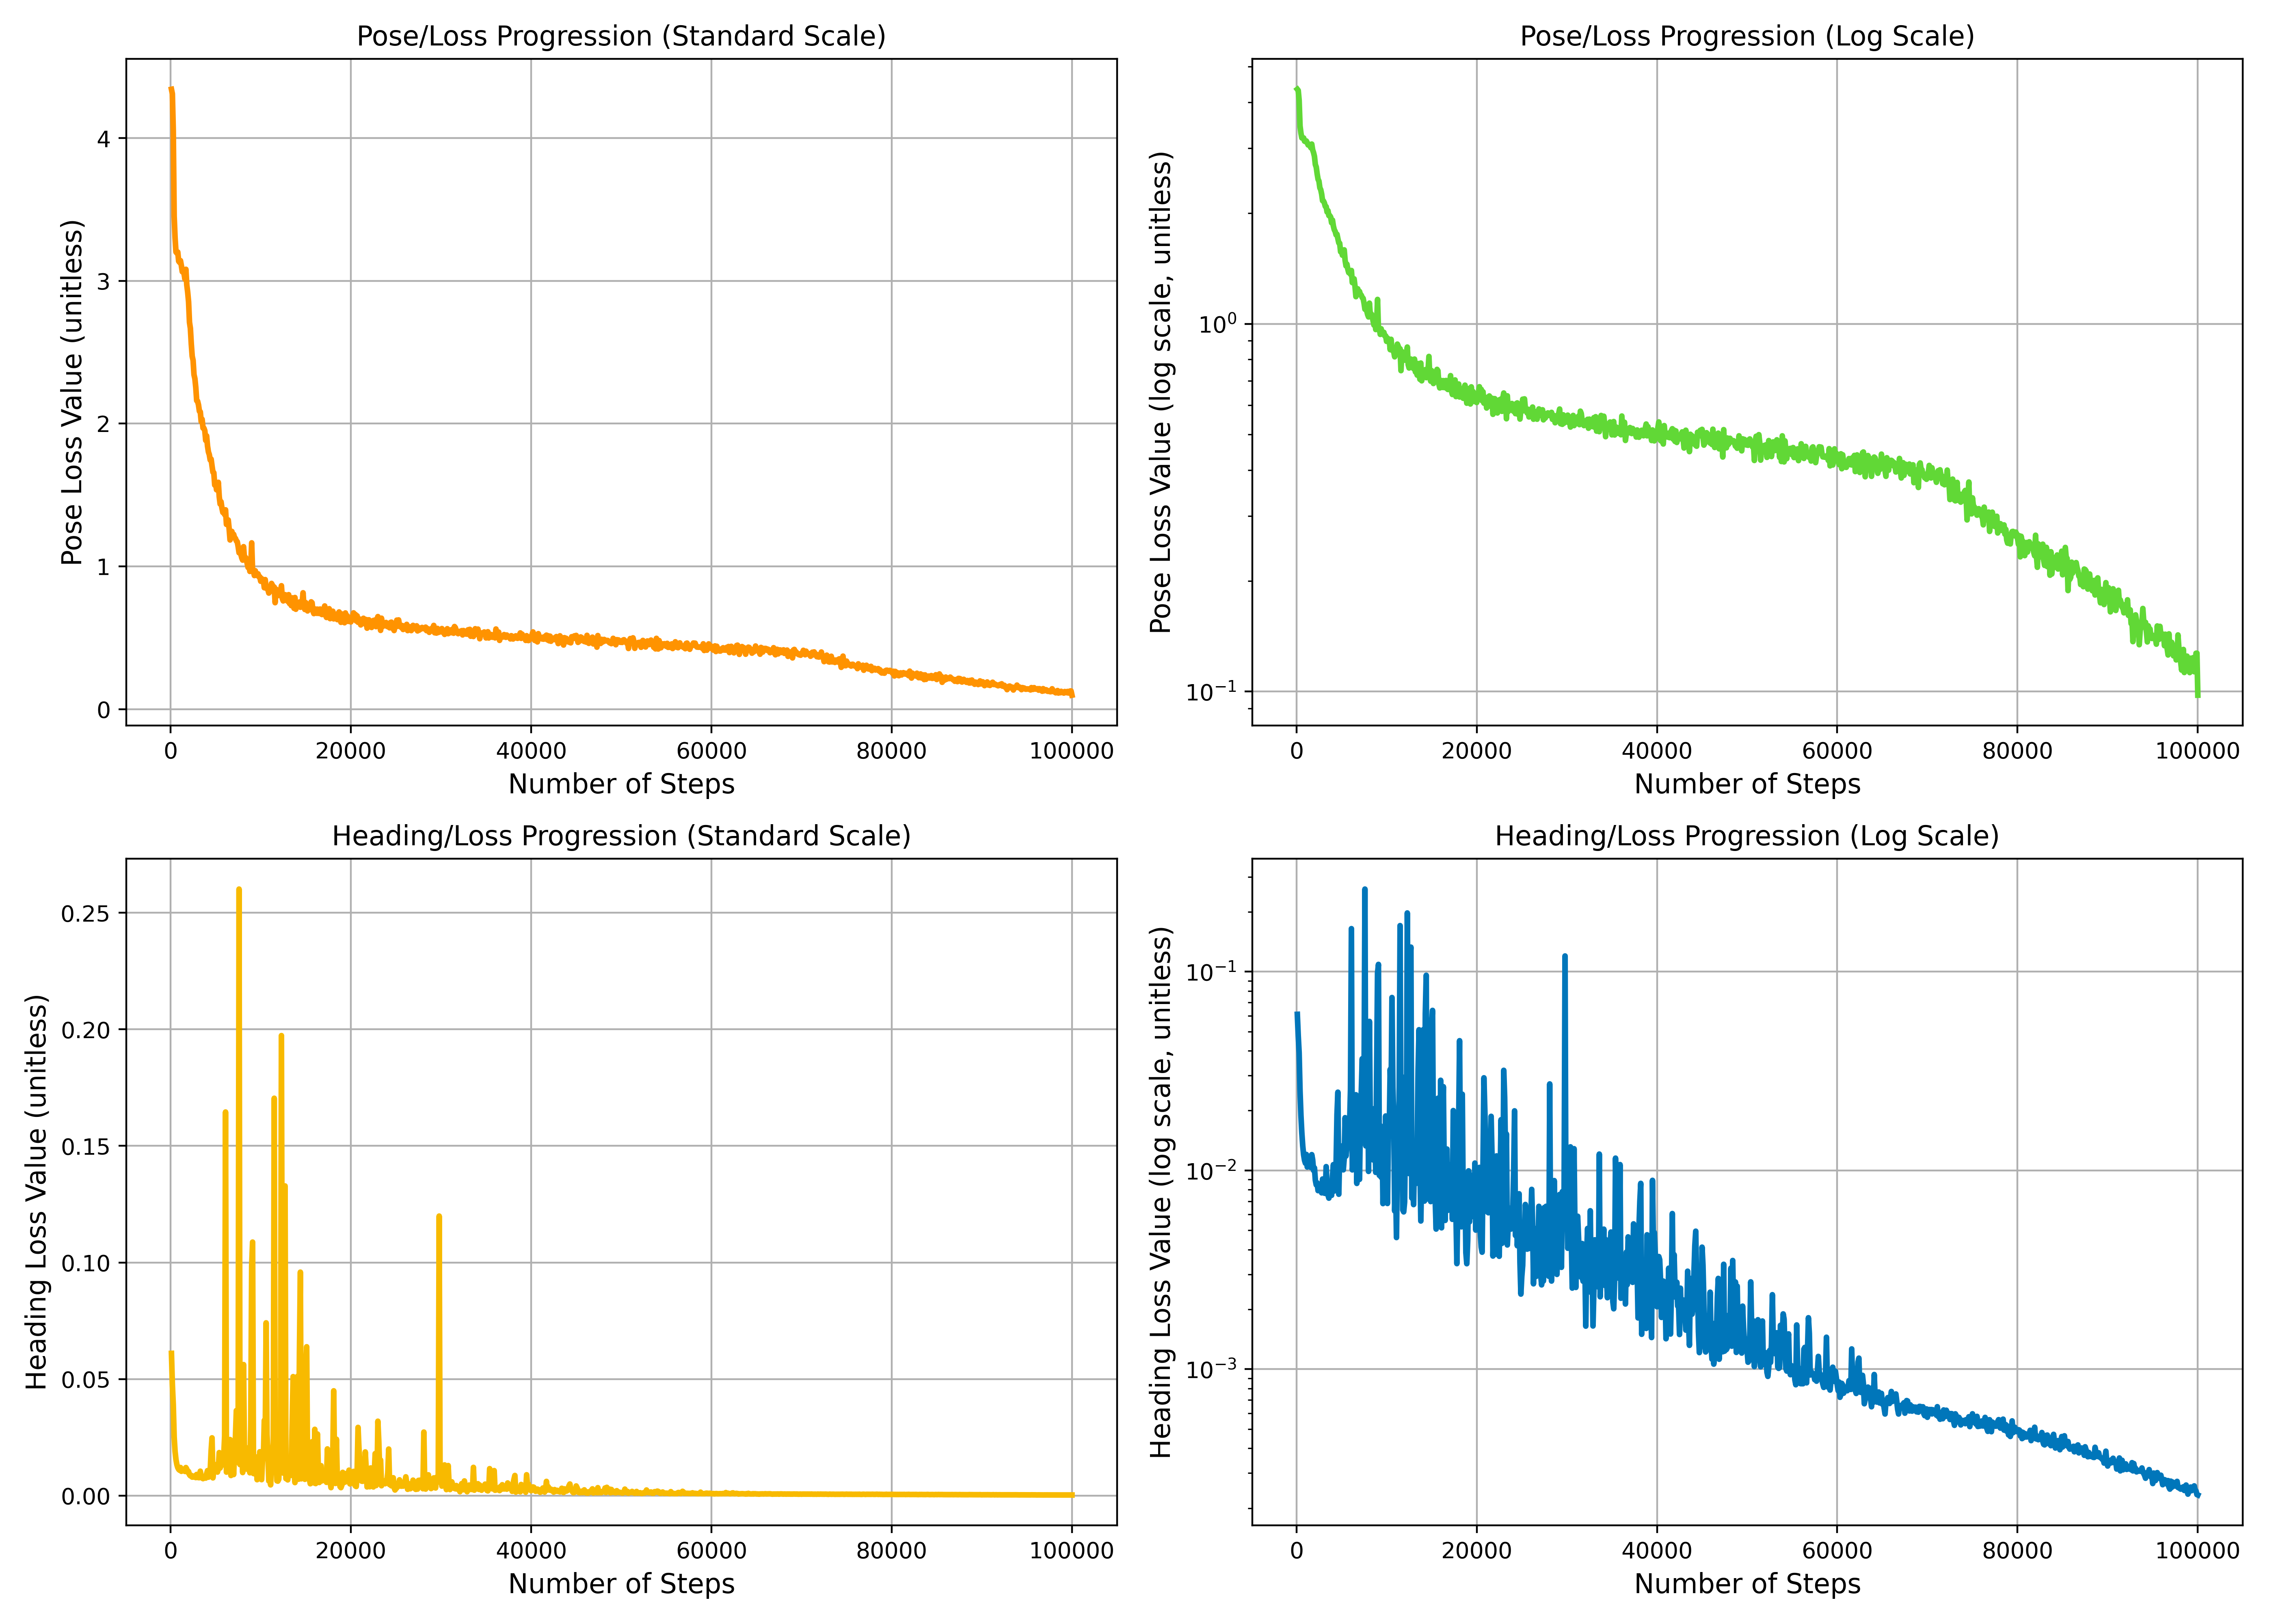
\includegraphics[width=1\linewidth]{LateX//figs/l1s_pose_heading_loss_comparison.png}
    \caption{Pose and Heading Loss Comparison Using Smooth L1 Loss}
    \label{fig:smooth-l1-pose-heading-loss}
\end{figure}

Below is reported a summary of the evaluation results observed during the training session:
\begin{table}[H]
    \centering
    \begin{tabular}{>{\centering\arraybackslash}p{2.25cm} >{\centering\arraybackslash}p{2.25cm} >{\centering\arraybackslash}p{3.25cm} >{\centering\arraybackslash}p{2.25cm} >{\centering\arraybackslash}p{2.25cm}}
        \toprule
        \textbf{Iteration} & \textbf{$\Delta$ Pose} & \textbf{$\Delta \theta$} & \textbf{$\Delta x + \Delta y$} & \textbf{$\Delta h$} \\
        & \text{[m]} & \text{[rad] $\rightarrow$ [deg]} & \text{[m]} & \text{[m]} \\
        \midrule
        \num{20000} & 1.75 & 0.14 $\rightarrow$ 8.02 & 1.72 & 0.02 \\
        \num{40000} & 1.81 & 0.14 $\rightarrow$ 8.02 & 1.72 & 0.02 \\
        \num{60000} & 1.35 & 0.02 $\rightarrow$ 1.15 & 1.36 & 0.01 \\
        \num{80000} & 1.46 & 0.02 $\rightarrow$ 1.15 & 1.46 & 0.00 \\
        \num{100000} & 1.38 & 0.02 $\rightarrow$ 1.15 & 1.28 & 0.00 \\
        \bottomrule
    \end{tabular}
    \caption{Variations in pose, angle, xy, and height across different iterations.}
    \label{tab:pose_variations}
\end{table}

The table shows that the Smooth L1 loss gave the best results. This makes sense because Smooth L1 combines the strengths of L1 and L2 losses. It handles outliers better than MSE loss while keeping a good balance between speed and stability during training. This makes it a good choice for regression tasks involving spatial transformations. However, the improvements from switching to Smooth L1 loss were not enough to achieve the level of precision needed for this specific task.

To ensure that all predicted values are comparable, it is important to have them on the same scale. This helps avoid issues where one variable dominates the loss function due to having larger values, while smaller-scaled variables are neglected. Additionally, keeping values on a similar scale improves the efficiency of the optimization process, as optimization algorithms like Adam or SGD perform better when variables are normalized or standardized. For this reason, the heading angle was converted from radians to degrees, aligning its scale with the three translation values, making them more comparable and ensuring balanced learning across all predicted outputs.
The same experiments were repeated after this adjustment, using the same loss functions, with results shown below.
\begin{figure}[H]
    \centering
    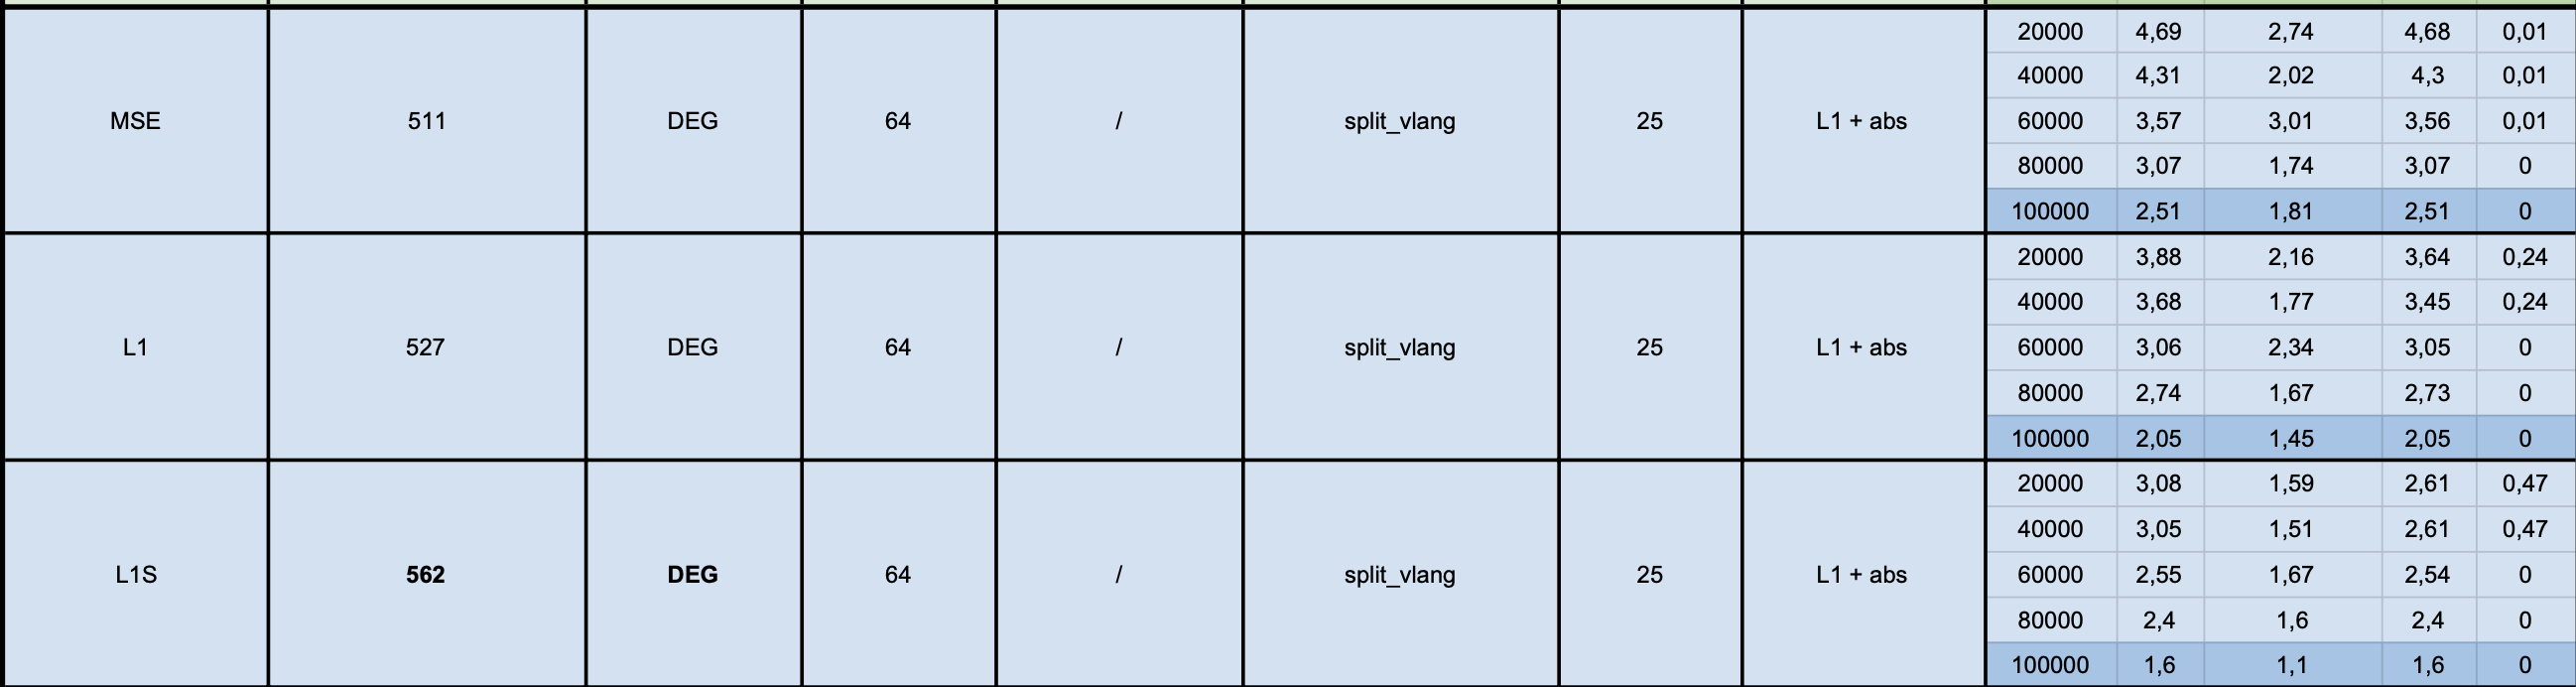
\includegraphics[width=1\linewidth]{Screenshot 2024-11-14 at 11.52.27.png}
    \caption{Evaluation Results with Heading Angle in Degrees (TABELLA DA RIFARE)}
    \label{fig:degree-evaluation-results}
\end{figure}

These results underscore the critical role of maintaining consistent value scales across predicted parameters and reaffirm the effectiveness of Smooth L1 loss in training this kind of models.
\begin{figure}[H]
    \centering
    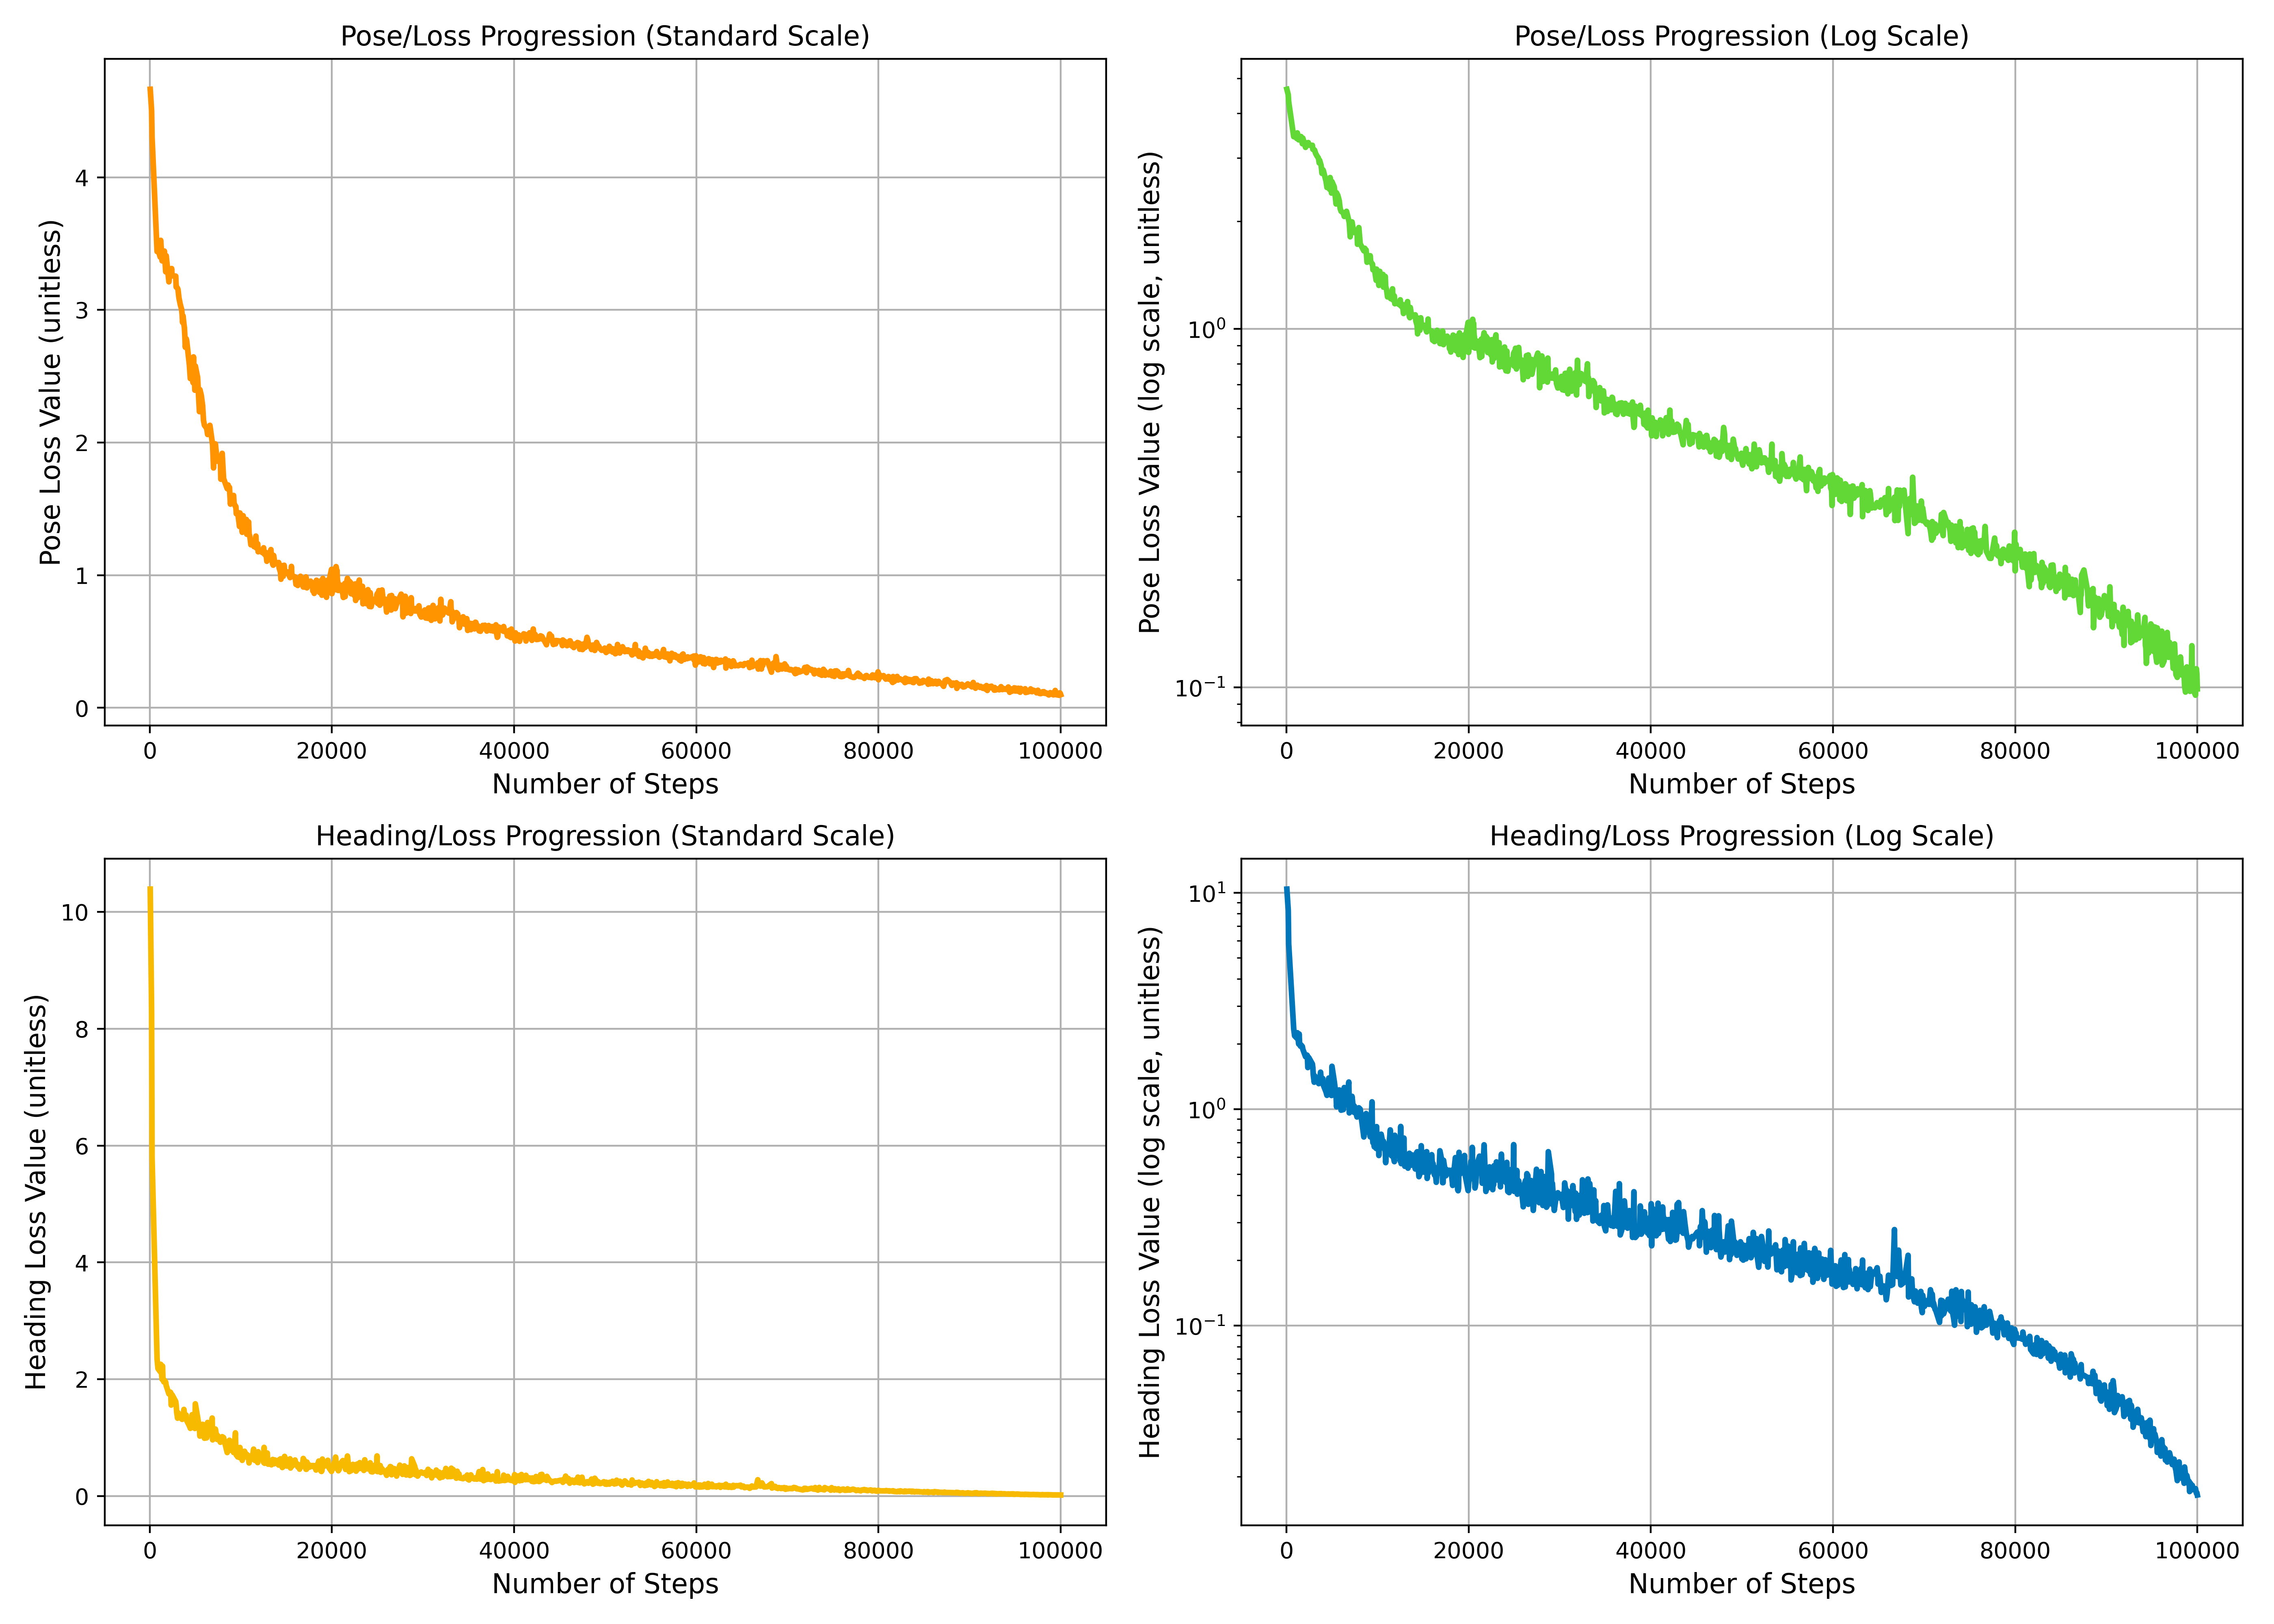
\includegraphics[width=1\linewidth]{LateX//figs/l1s_111_DEG_pose_heading_loss_comparison.png}
    \caption{Enter Caption}
    \label{fig:enter-label}
\end{figure}

Converting the heading angle to degrees, as expected, led to improved results by reducing errors and aligning predicted values more closely with the desired targets. Once again, the Smooth L1 loss demonstrated superior generalization performance.

As mentioned at the beginning of the sections, the above attemps were not done with all the dataset that could be used.
Given these findings, when the full dataset was utilized by merging all sequences from the three streets, only the best-performing model from the preliminary analysis (using Smooth L1 loss) was tested. The results are shown and discussed below.

\textbf{Full Dataset Results:} The figures below illustrate the improvements in angle prediction, which are attributed to the increased dataset size, the application of Smooth L1 loss, and the conversion of angles to degrees. Despite these advancements, significant challenges persist in addressing translation errors. While the current approach shows promise and demonstrates improvements, achieving precise HD map alignment will likely require further model refinement or still using the implementation of optimization techniques. This model version has the potential to assist in complex scenarios, but it does not fully resolve the alignment challenge.
\begin{figure}[H]
    \centering
    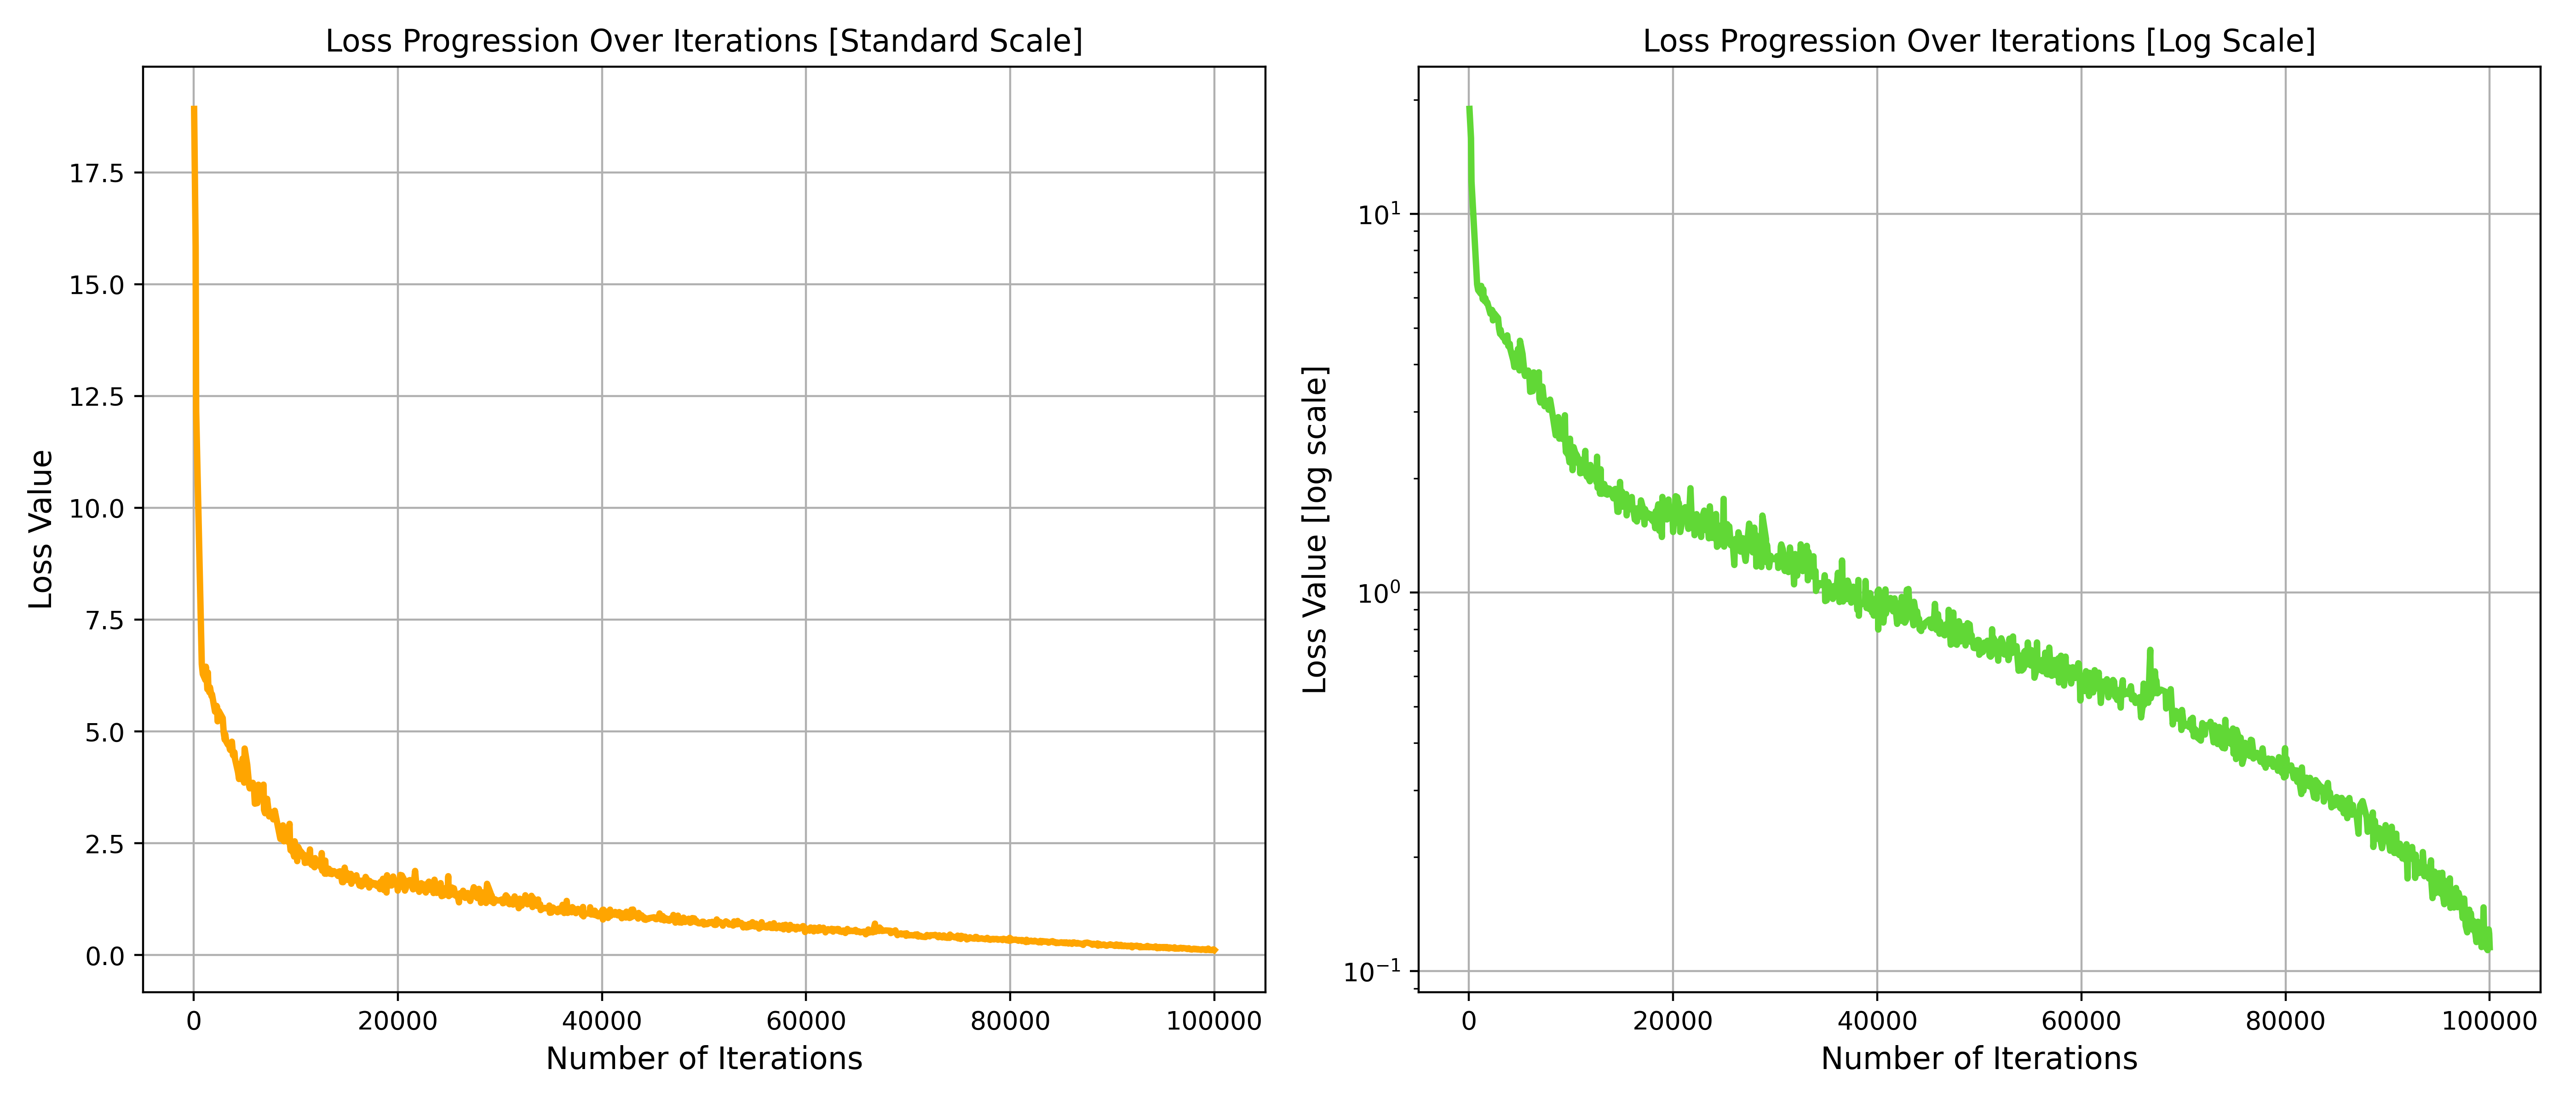
\includegraphics[width=1\linewidth]{loss_total_l1sDEG_progression_comparison.png}
    \caption{Progression of total loss with Smooth L1 loss (in degrees).}
    \label{fig:total-loss-progression}
\end{figure}

The results indicate that the contributions of heading and translation errors are approximately balanced in this case, which may explain the observed improvements in heading accuracy.
\begin{figure}[H]
    \centering
    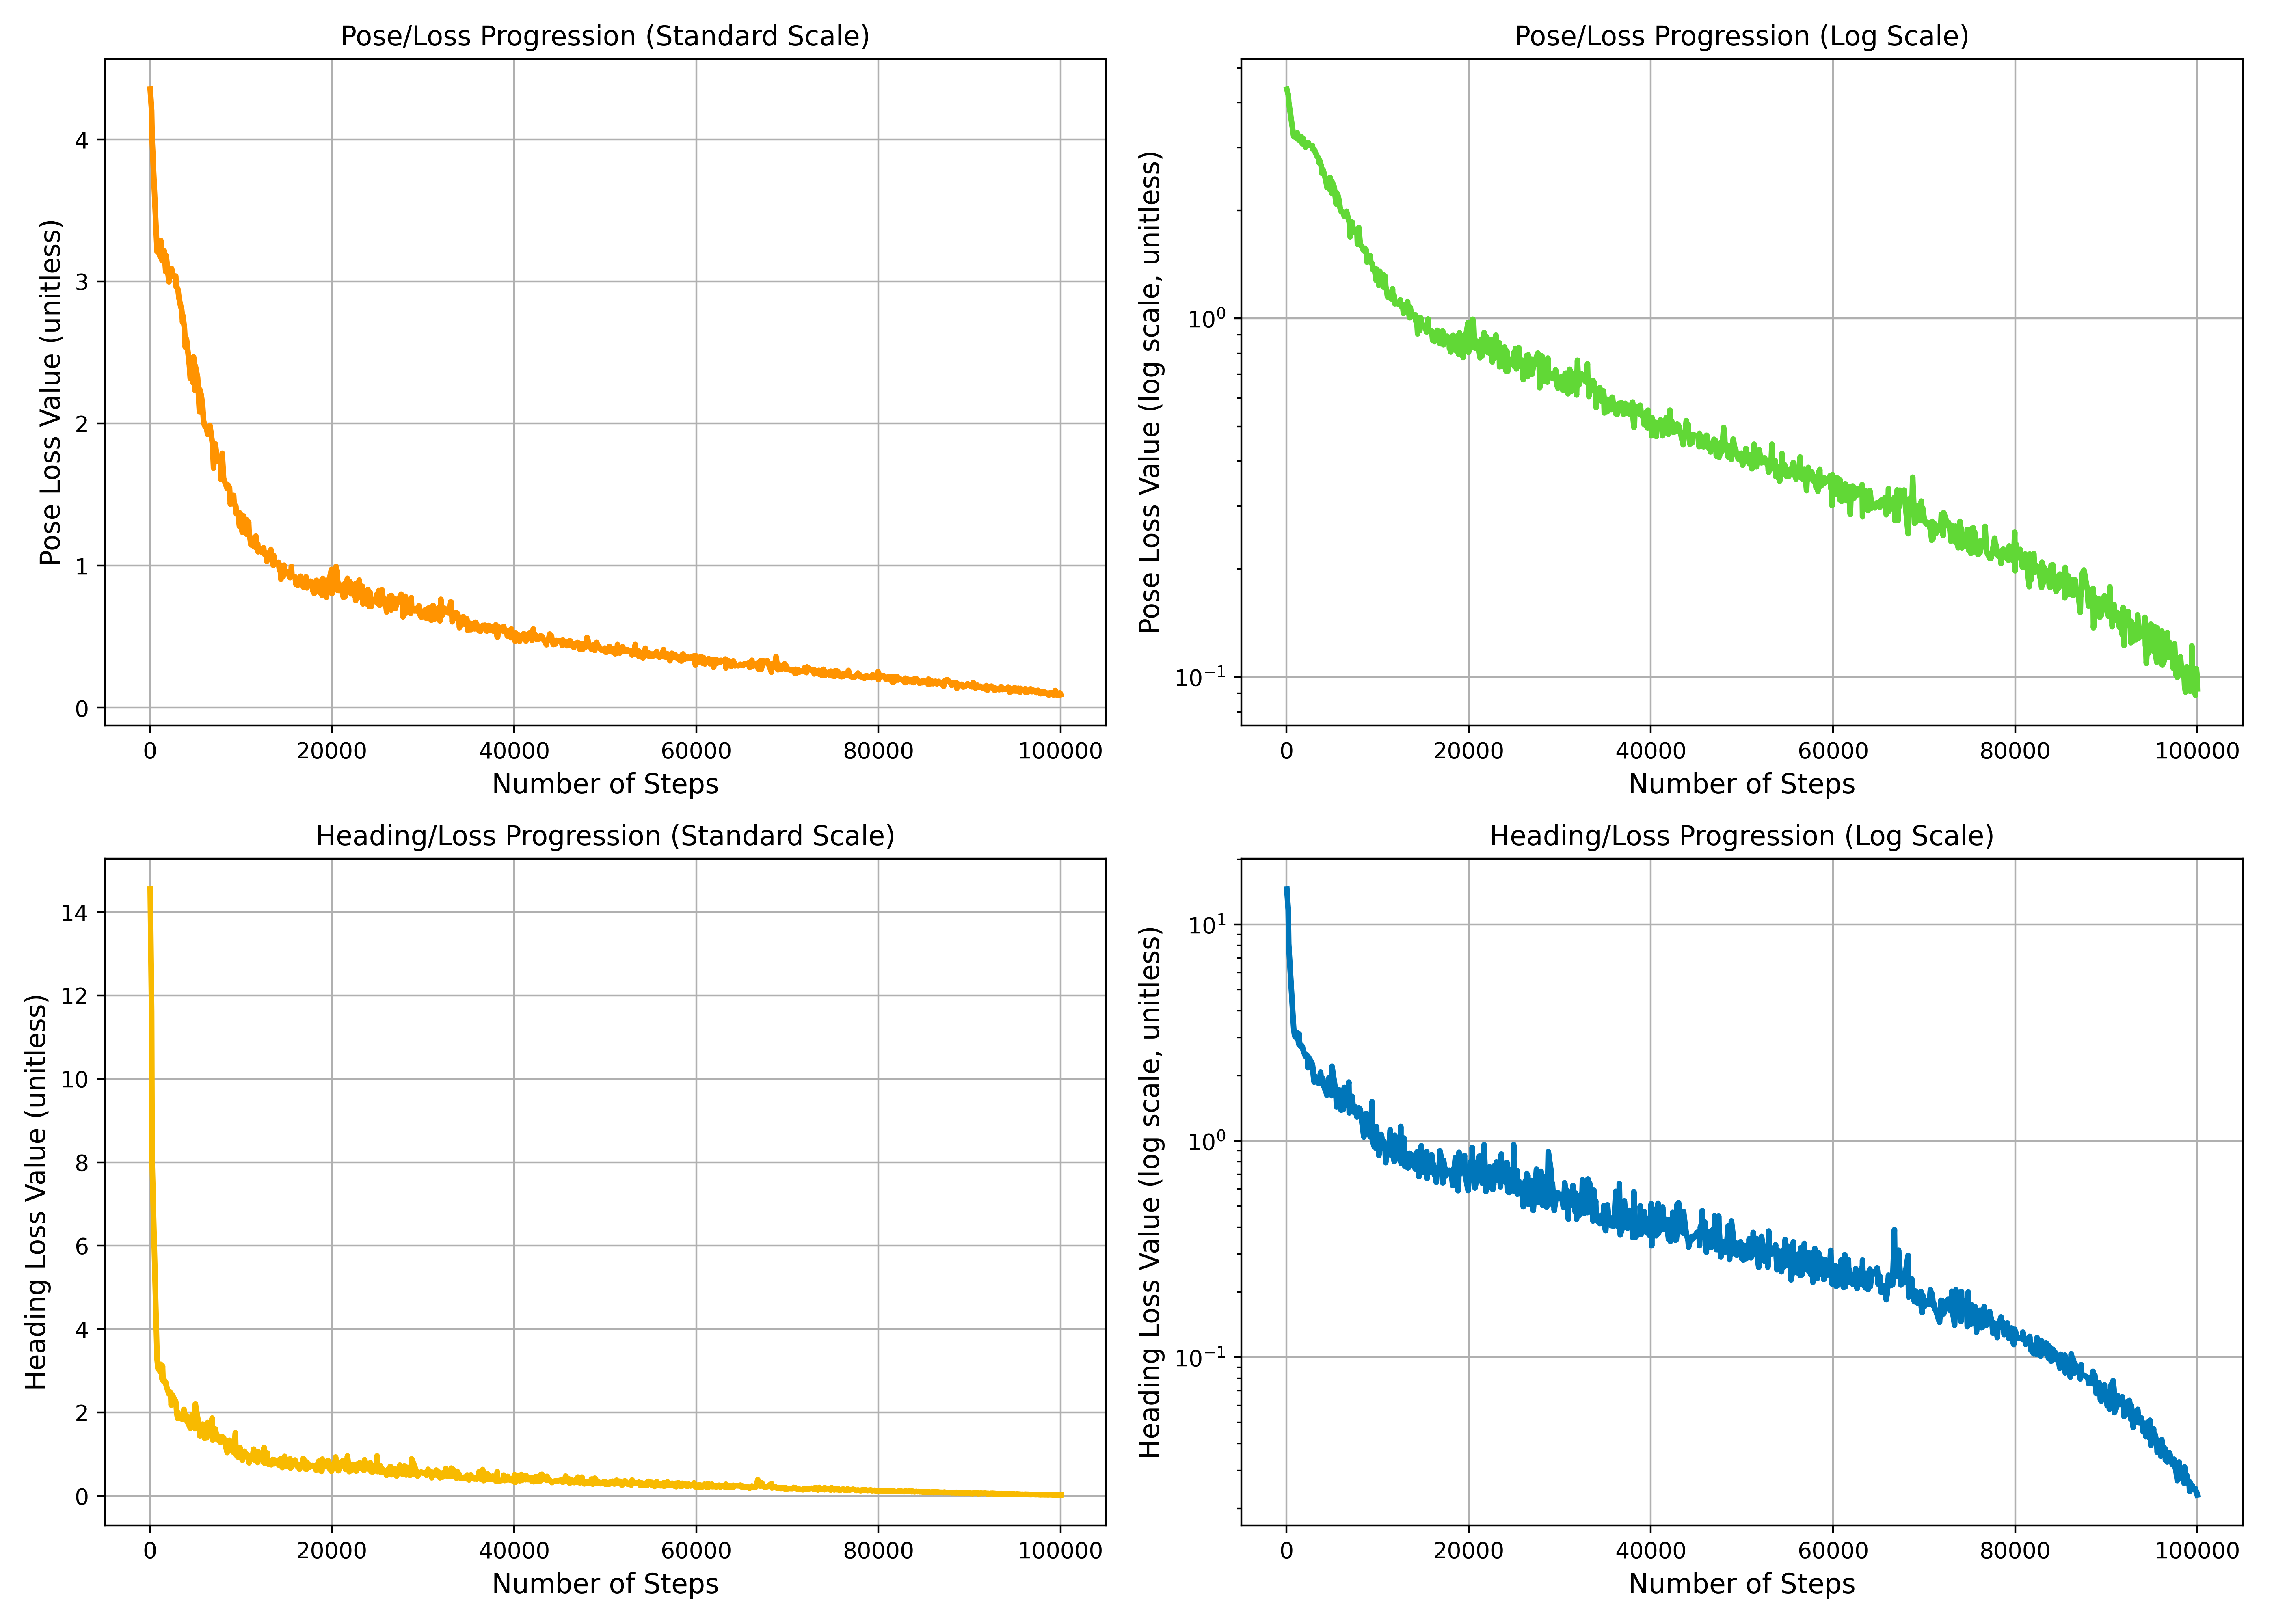
\includegraphics[width=1\linewidth]{LateX//figs/l1sDEG_pose_heading_loss_comparison.png}
    \caption{Comparison of pose heading loss across different iterations.}
    \label{fig:pose-heading-loss}
\end{figure}

A summary of the results obtained during different evaluation stages, as iterations progress, is provided in the table below.
\begin{figure}[H]
    \centering
    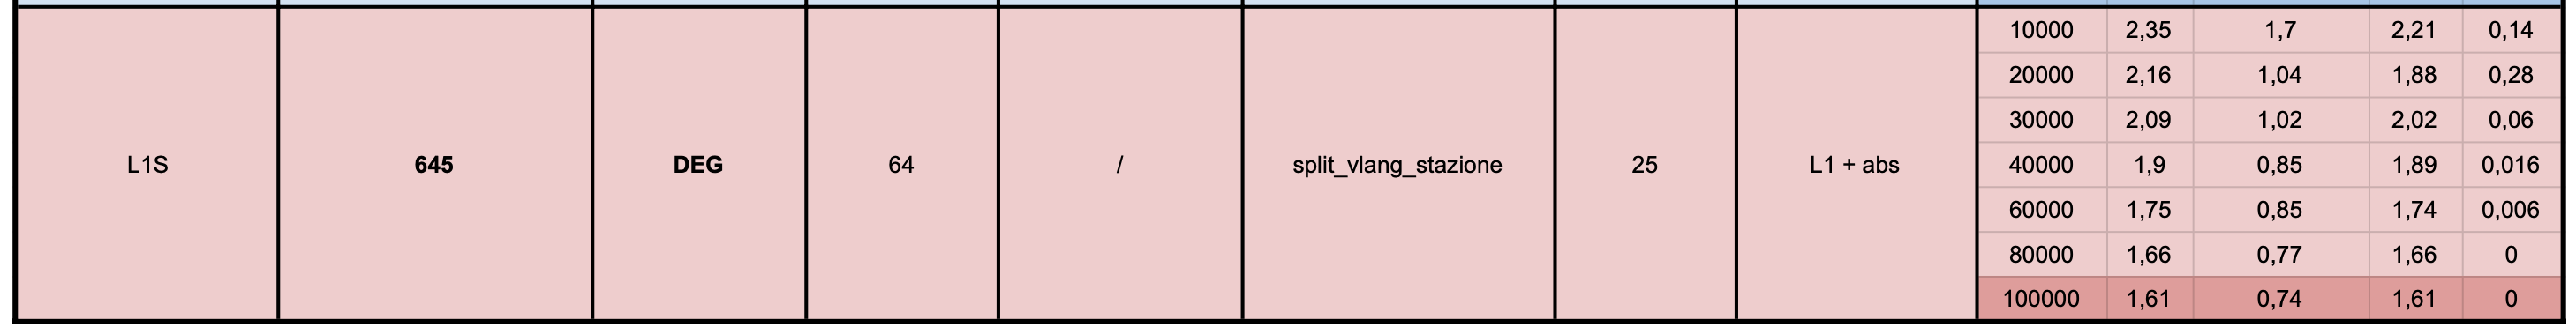
\includegraphics[width=1\linewidth]{LateX//figs/Screenshot 2024-11-15 at 14.26.05.png}
    \caption{Summary of evaluation metrics (DA RIFARE).}
    \label{fig:evaluation-summary}
\end{figure}

\subsection{Inference}
Inference was tested on a new sequence that was not included in the training dataset. This sequence mainly consisted of long, straight roads with few textures or reference points for alignment. The weights used for this test came from the most accurate model analyzed earlier.

During inference, the roto-translation between the map and the car was still applied using data augmentation. This allowed for a visual comparison between the expected target and the predicted results.

The results showed that the network tried to reduce the distance but started from the wrong boundary. This led to a good alignment of the angle but caused the translation to be misaligned by the width of an entire lane. This issue is similar to what can occur with classical optimization methods and represents a scenario that should be avoided. The misalignment is consistent with the evaluation results observed during different stages of training.
The figure below follows the same layout as before, showing the input, the target, and the final prediction in three vertical panels. In this case, the values were not post-processed, so the roto-translation was applied directly to the map instead of the car.

\begin{figure}[H]
    \centering
    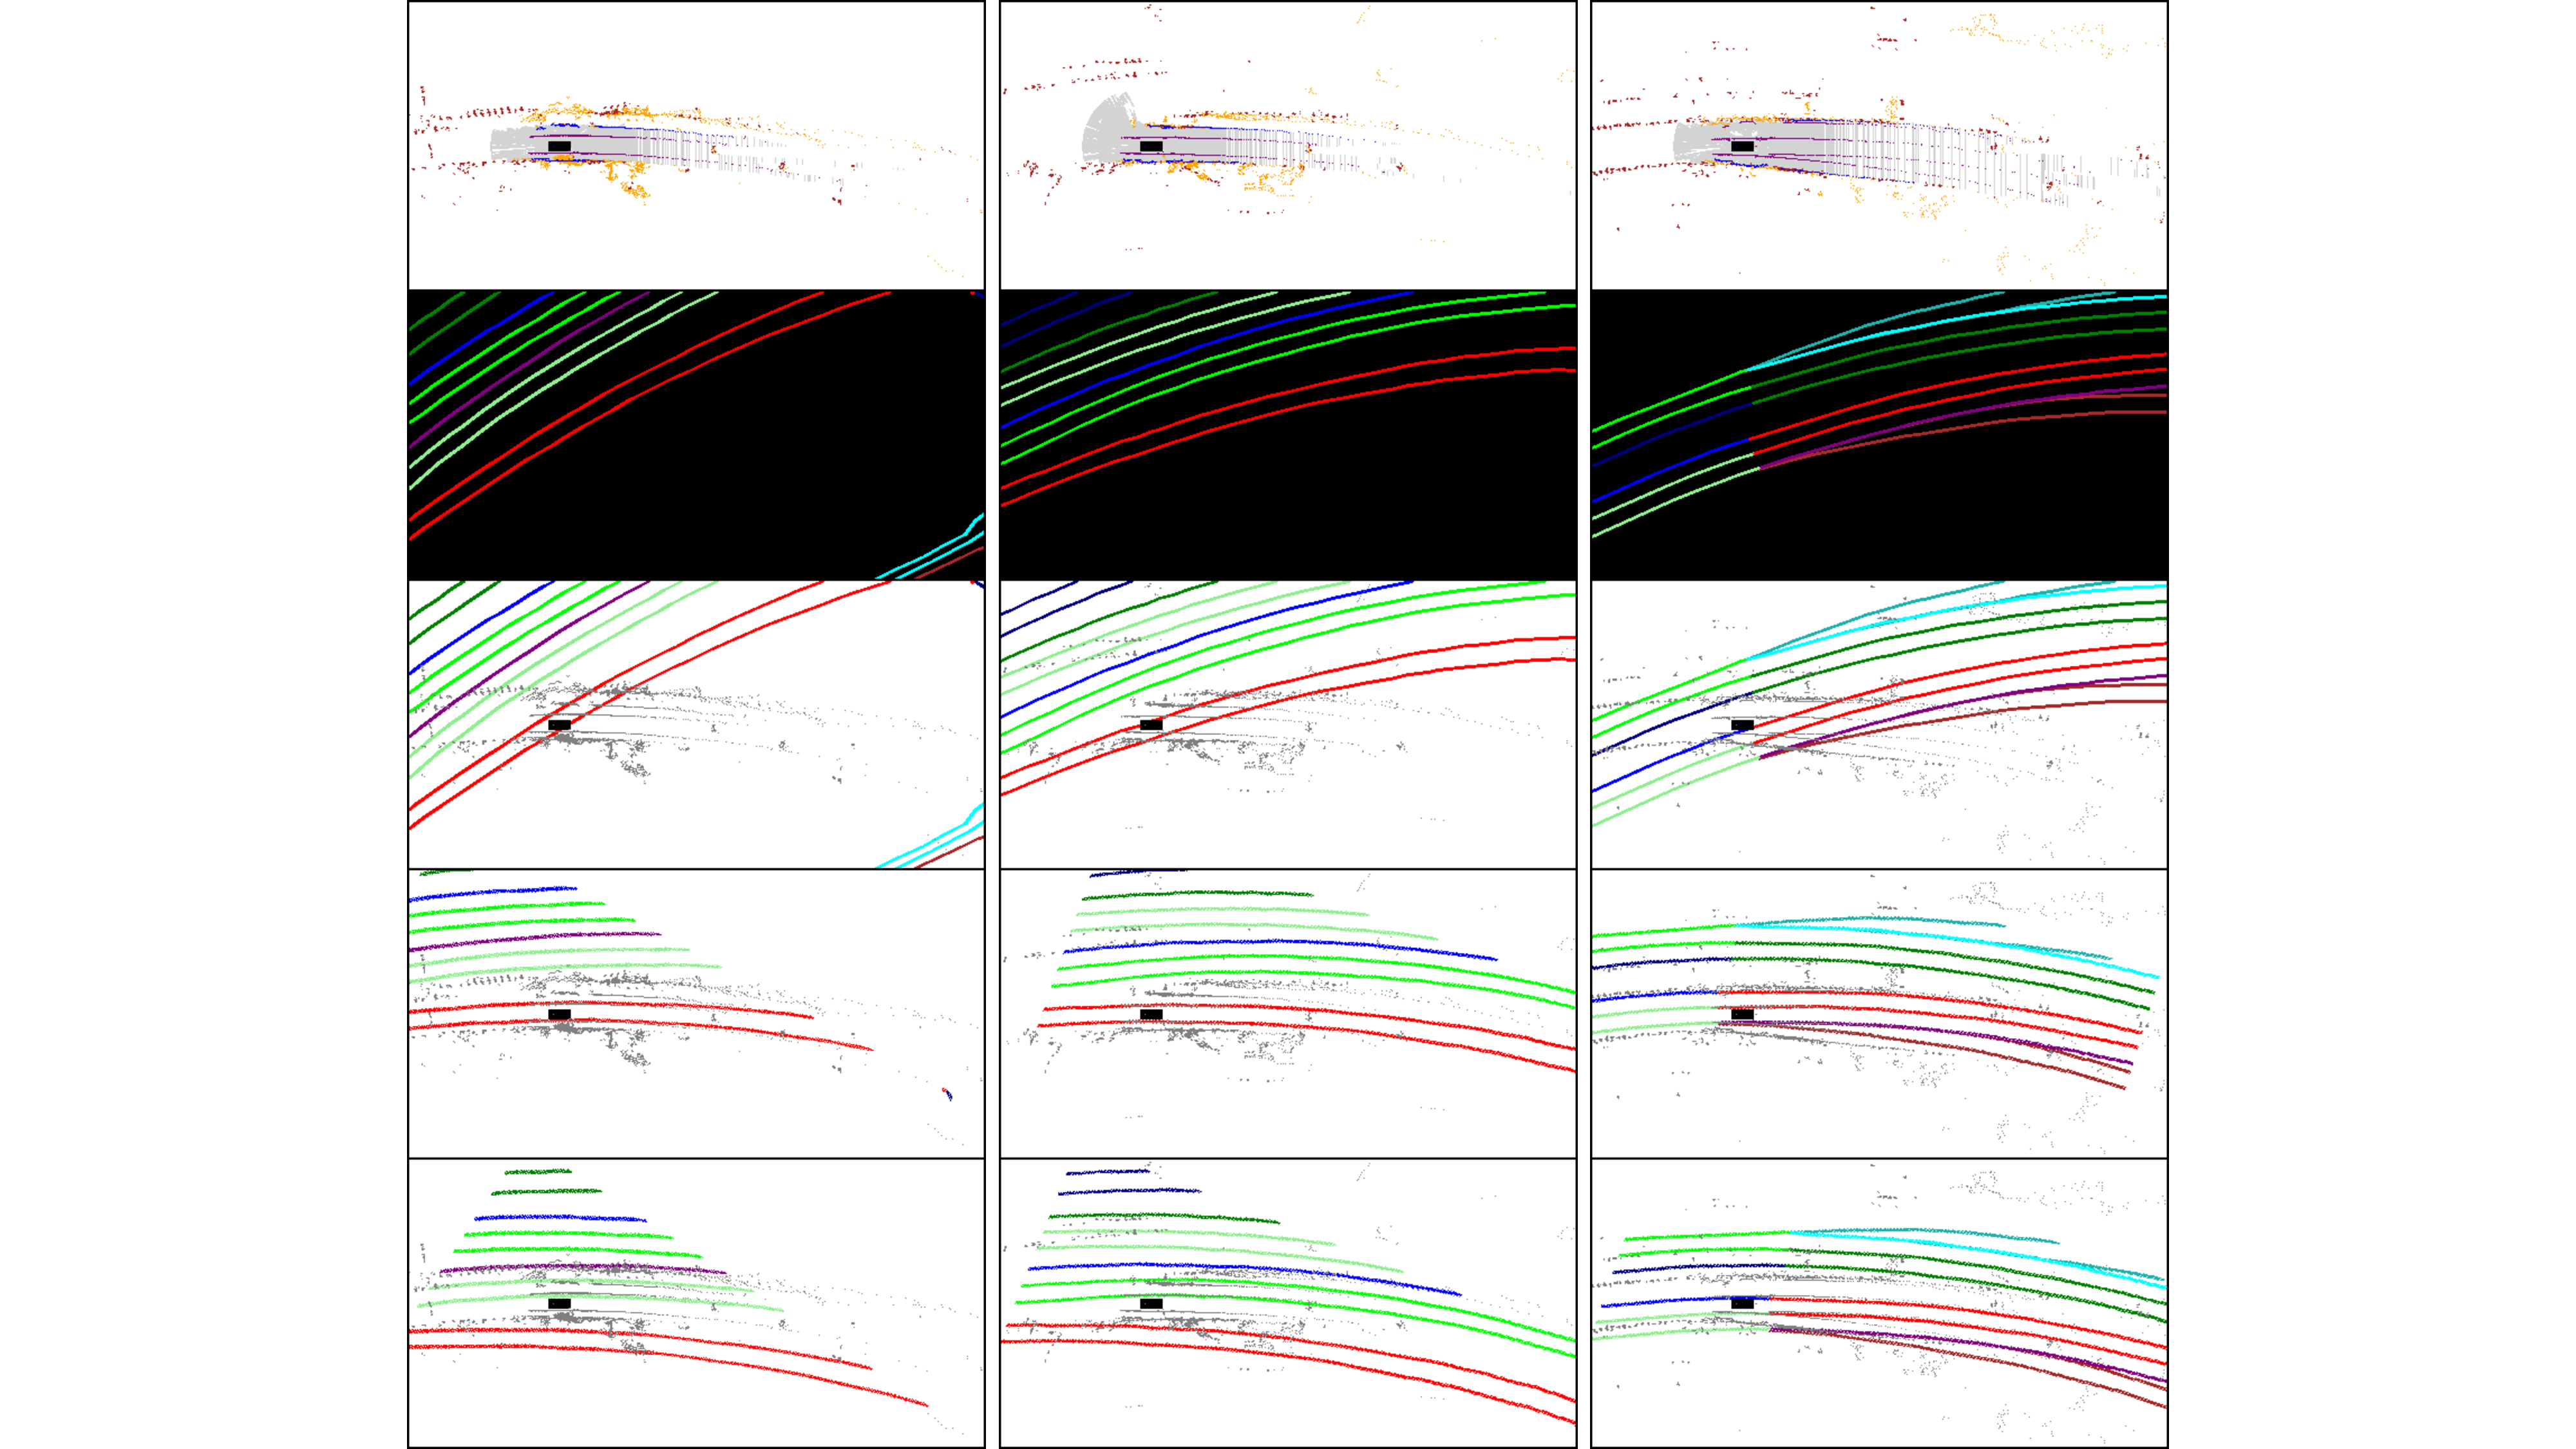
\includegraphics[width=1\linewidth]{Untitled 2.pdf}
    \caption{Example of inference results showing angle alignment but translation error.}
    \label{fig:inference-results}
\end{figure}

\section{Second Approach}
\subsection*{Smooth L1 Loss}
\subsection{Inference}